\documentclass{BachelorBUI}
\usepackage[utf8]{inputenc}
\RequirePackage[babel,english]{csquotes} %% context sensitive quotations
\raggedbottom
\lstset{
 language={Matlab},
}
\sisetup{output-decimal-marker = {.},
range-phrase = --,
group-separator = {,},
per-mode = symbol,
list-final-separator={ and }}

%----------------------------------------------------------------------------------------
% Packages
%----------------------------------------------------------------------------------------
\usepackage{tikz}
\usepackage{color}
\usetikzlibrary{positioning, shapes.multipart}

%----------------------------------------------------------------------------------------
% Graphics
%----------------------------------------------------------------------------------------
\graphicspath{{images/}}

%----------------------------------------------------------------------------------------
% New commands and other new definitions (e.g. colors)
%----------------------------------------------------------------------------------------
\newcommand{\eg}{\mbox{e.\,g.}\xspace}
\newcommand{\Name}[1]{\textsc{#1}}
\newcommand{\abs}[1]{\left|#1\right|}
\colorlet{light_grey}{gray!25}
\colorlet{dark_grey}{light_grey!50!black}
\colorlet{light_red}{red!25}
\colorlet{dark_red}{light_red!50!black}
\colorlet{light_blue}{blue!25}
\colorlet{dark_blue}{light_blue!50!black}
\colorlet{light_green}{green!25}
\colorlet{dark_green}{light_green!50!black}

%----------------------------------------------------------------------------------------
% Acronyms
%----------------------------------------------------------------------------------------
\usepackage{acro}
\acsetup{list/display=used}
\input{acronyms}

%----------------------------------------------------------------------------------------
% Settings of document structure depth
%----------------------------------------------------------------------------------------
\setcounter{secnumdepth}{3}
\setcounter{tocdepth}{3}

%----------------------------------------------------------------------------------------
% Bibliography
%----------------------------------------------------------------------------------------
\usepackage[style=authoryear,backend=biber,maxcitenames=2]{biblatex}
\ExecuteBibliographyOptions{%
 giveninits=true, maxbibnames=99}%
\DefineBibliographyStrings{english}{%
andothers={et\;al\adddot},
urlseen = {Accessed on}
}
\addbibresource{references.bib}
\setcounter{biburllcpenalty}{9000}% Lowercase
\setcounter{biburlucpenalty}{9000}% Uppercase

%----------------------------------------------------------------------------------------
% Title and author information
%----------------------------------------------------------------------------------------
\title{Plant Disease Classification:\\[0.5em]\LARGE An Approach using Convolutional Neural Networks}
\authorname{Jakub Dunaj}
\email{e12121285@student.tuwien.ac.at}
\MatrNr{12121285}
\thesislanguage{en-US}
\keywords{bachelor's thesis\sep plant disease classification\sep convolutional neural networks\sep CNNs\sep}

%----------------------------------------------------------------------------------------
% Begin of the document
%----------------------------------------------------------------------------------------
\begin{document}
\selectlanguage{english}
\begin{filecontents}[overwrite]{\jobname.xmpdata}
\makeatletter
\Title{\@title}
\Author{\@authorname}
\Language{\@thesislanguage}
\Keywords{\@keywords}
\Publisher{TU Wien}
\makeatother
\end{filecontents}

%----------------------------------------------------------------------------------------
% Title
%----------------------------------------------------------------------------------------
\maketitle

%----------------------------------------------------------------------------------------
% Abstract
%----------------------------------------------------------------------------------------
\begin{abstract}
\end{abstract}

%----------------------------------------------------------------------------------------
% Table of contents
%----------------------------------------------------------------------------------------
\clearpage
\tableofcontents

%----------------------------------------------------------------------------------------
% Bachelor's thesis
%----------------------------------------------------------------------------------------
\clearpage
\section{Introduction}

% climate change \cite{Sladojevic:2016}

\section{Thesis Focus and Related Research}

    This section is divided into two main parts. The first part gives an overview of machine learning, describes different machine learning approaches and gives detailed insights into neural networks, especially into convolutional neural networks. The second part presents and reviews related research in the field of plant disease classification from leaf images.

    \subsection{Machine Learning: An Introduction}
    \label{sec:machine-learning-overveiw}

        The reader of thesis thesis may think about a random sequence of characters 'd' and 'f'. Next, the reader can try to write down a random sequence of maybe 10 to 20 of these two characters. How random does the reader think the sequence is? Are there any patterns present in the sequence? In fact, this is hard to tell only from one short sequence. What about thousand sequences or one very long sequence? Does the reader think that those would be random and unique even if trying very hard? I would advise the reader to have a look at the following website \url{https://people.ischool.berkeley.edu/~nick/aaronson-oracle/index.html} and try the website out. The algorithm on the website attempts to predict whether the next typed character will be 'd' or 'f'. The algorithm predicts the next typed character based on the sequence of 'd's and 'f's the user has typed so far. In \autoref{fig:website-predicting-typed-characters}, the algorithm could predict user's next typed character with a probability of 67\%.

        \begin{figure}[h]
            \centering
            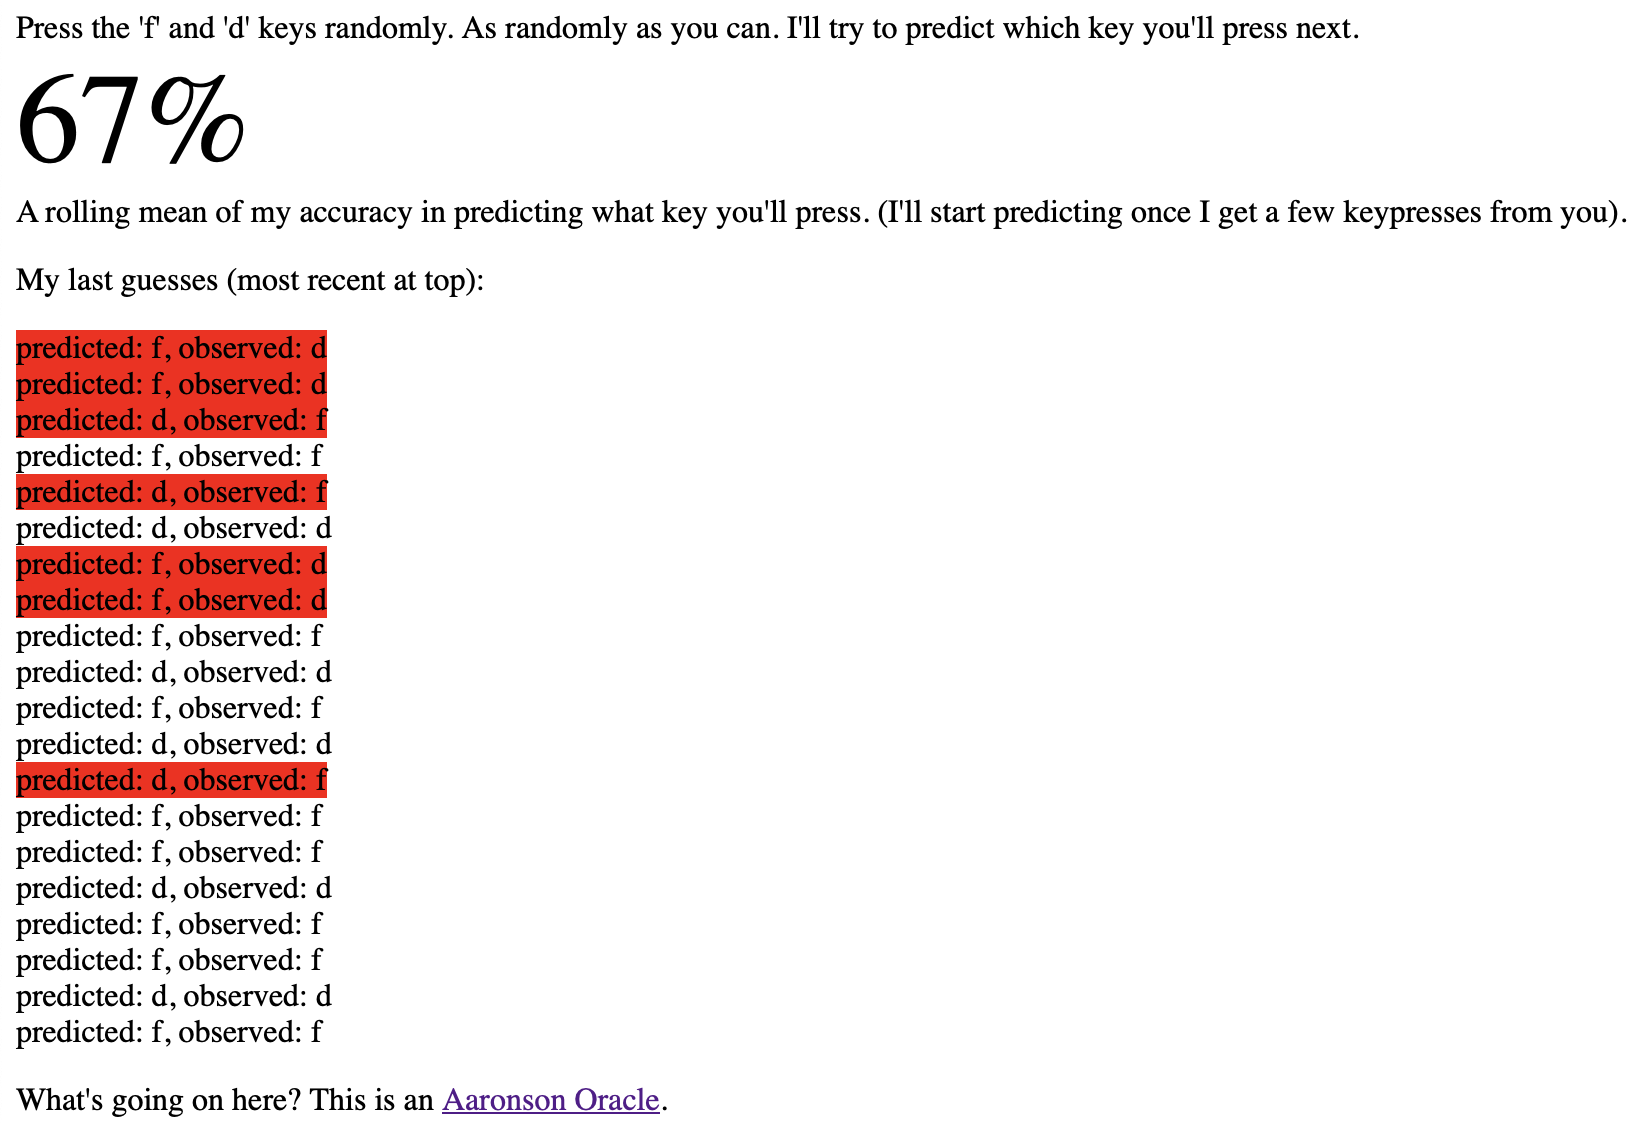
\includegraphics[width=0.8\textwidth]{website_predicting_typed_characters.png}
            \caption{\centering Website predicting whether the user will type 'd' or 'f' next (\cite{website_predicting_typed_characters:2024})}
            \label{fig:website-predicting-typed-characters}
        \end{figure}

        The website is based on the book "Quantum Computing since Democritus" by Scott Aaronson. \textcite{Aaronson:2013} wrote a simple program predicting whether the next typed character would be 'd' or 'f'. The author found that the algorithm was successful 70\% of the time. To answer the rhetorical questions asked at the beginning of this sections, humans can't generate truly random sequences of 'd's and 'f's. There is something fundamental in our sequences making the next character predictable. That is true for all human-generated data. In fact, we leave patterns in all our data. This is tightly coupled with human behavior and the complexity of our everyday tasks. Humans don't behave randomly. We exercise different behavioral patters instead. We can observe this phenomenon all around us. For example, fashion trends differ between generations or age groups. Young people wear different styles of clothes than elderly people. People with higher income spend their money differently than people with lower income. Sporty people are maybe more health conscious and tend to buy healthier groceries than general population.

        We can think, for example, of a large fashion retailer offering thousands of articles in thousands of physical stores and through a website. This retailer wants to know which products or styles and when are popular among customer. The retailer stores different data from every transaction made online or in-store by customers enrolled in the bonus program: customer gender, customer age, articles bought, total price, store location, current weather, current clothing season, and many others. Customers don't buy their clothes randomly. They are influenced by many different factors, such as their gender or age group. From this huge amount of collected data, the retailer could infer different behavioral patterns and accordingly modify its offer to maximize profits. The retailer could ask the following question: "What products do 35-year-old customers buy in Vienna during the summer after 2PM?". Clearly, there is no standard algorithm for this complex multidimensional problem. We don't have the knowledge about the behavioral patterns of the customers. Instead, we need to create a mechanism that would infer these patterns in customers' buying habits from the transaction data. That is where the machine learning comes into play. It allows us to predict possible outputs based on a specific input of parameters. In the specified problem, the input parameters would be the customer's age, store location, clothing season and purchase time. We would expect the mechanism to predict the customers' preferences from these input parameters. The mechanism would obtain and infer the knowledge from the transaction data.

        More formally, we can define machine learning as creating and applying computational methods using data to make accurate predictions or optimize different complex tasks (\cite{Mohri:2018}). These computational methods consist of learning algorithms processing the training data and models representing the knowledge gained from the learning process (\cite{Alpaydin:2014}). A model is defined by a set of parameters influencing model's response to a given input (\cite{Alpaydin:2014}). A model can be, for example, simple linear function or a complex model such as a neural network. During the learning process, the learning algorithm optimizes model's parameters using the training data (\cite{Alpaydin:2014}). The final trained model approximates the patterns and regularities present in the data and provides useful representation of the knowledge gained during the training process (\cite{Alpaydin:2014}). We can refer to the training data as the experience the training algorithms use to train machine learning models. A trained model may not contain all information present in the training data, but it makes predictions that are accurate enough and thus useful (\cite{Alpaydin:2014}). From the computer science perspective, there are different aspects of machine learning that have to be considered (\cite{Alpaydin:2014}). The learning algorithm must efficiently solve the optimization problem of model's parameters. There must be an efficient way to store and process large amounts of training data, and the model's algorithmic representation must be efficient as well.

        Machine learning is a subfield of artificial intelligence. To be and behave intelligent, a machine learning model has to have the ability to learn and adapt to the changes in the training data (\cite{Alpaydin:2014}). The changes in the training data result from the changes in the experience the data describes. The model has to adapt to these changes through learning to accurately approximate the experience. Furthermore, because of the ability of the machine learning models to learn and adapt, there is no need to program the model explicitly (\cite{Alpaydin:2014}). The trained model may be predictive, descriptive, or have both of the features at the same time (\cite{Alpaydin:2014}). This means that the model can make predictions about the future or describe the knowledge from the data, or even do both. All the model's knowledge is inferred from the training data.

        The prediction accuracy of a model depends on the size of training data and the model complexity (\cite{Murphy:2022}). A model is accurate when it can generalize well (\cite{Mohri:2018}). Generalization means that the model makes accurate predictions not only about the training data but also about unseen data (\cite{Bishop:2006}). To achieve good model generalization, a trade-off between the size of the training data and the model complexity must be done (\cite{Bishop:2006,Mohri:2018}). The model complexity can be defined as the number of parameters of the model (\cite{Bishop:2006}). When the training data is small and the model is too complex, it may generalize poorly on unseen data (\cite{Mohri:2018}). This is known as overfitting of the trained model (\cite{Mohri:2018}). On the other hand, a model that is too simple may not be able to achieve sufficient accuracy on the training data. This is known as underfitting (\cite{Mohri:2018}).

        What kind of problems can be solved using machine learning? When do we use machine learning instead of explicitly programming a computer program? There are two aspects of the problems we have to consider. These are the complexity of the problem and the need for adaptivity of the computer program (\cite{Shalev-Shwart:2014}). Complex problems may require mimicking animal or human intelligence or even go beyond human capabilities (\cite{Shalev-Shwart:2014}). The adaptivity of the computer program is its ability to learn from a changing experience without explicit programming (\cite{Shalev-Shwart:2014}). Machine learning is used in a variety of problem settings that involve: natural language processing, speech processing, computer vision, computational biology, and many others (\cite{Mohri:2018}).

        The following part of this section discusses machine learning approaches and neural networks as a machine learning model. It also gives an overview of neural networks because they play a central role in this thesis.

        \subsubsection{Machine Learning Approaches}

            Machine learning approaches can be divided into different categories based on the type of experience machine learning algorithms use to train machine learning models (\cite{Goodfellow:2016}). The different categories of machine learning approaches are: supervised, unsupervised and reinforcement learning. These categories are groups of machine learning algorithm that use the same type of experience for the training of models. As mentioned in the previous sections, the experience is the training data used by a machine learning algorithm. Each of these categories of machine learning algorithms can be applied to different groups of learning problems. Next, the different categories of machine learning algorithms and also the groups of learning problems the categories of algorithms are used for.

            \paragraph{Supervised Learning}

                In supervised learning, the objective is to train a machine learning model using labeled training data to map an input to a correct output (\cite{Alpaydin:2014}). This learning approach is called supervised because the training data consists of input--output pairs (\cite{Murphy:2022}). This means that the output is known for every input. The input of a machine learning algorithm is called a feature, which is typically a fixed-dimensional vector of numbers (\cite{Murphy:2022}). The output of a trained model is typically also a fixed-dimensional vector (\cite{Bishop:2006}). A machine learning algorithm uses the input vector from the problem instance to train a model that maps this input to an output vector (\cite{Bishop:2006}). An output that is associated with an input is also known as a label (\cite{Murphy:2022}). During a supervised learning process of a machine learning model, a machine learning algorithm tries to minimize the approximation error between the true label and the label predicted by the trained model (\cite{Alpaydin:2014}). A machine learning algorithm does this by adjusting the parameters of the trained model (\cite{Alpaydin:2014}). A feature used by a machine learning algorithm could be a vector of values representing pixels of an image (\cite{Murphy:2022}). The label of such an input vector could be the name of an object that is represented in the image.

                There are two different groups of machine learning problems that can be solved using a supervised learning approach: classification and regression problems. In classification problems, every problem instance belongs to a class. The task in classification problems is the prediction of the class of a problem instance (\cite{Goodfellow:2016}). In supervised learning, the problem instance and its associated class build the input--output pair. The output of a machine learning model trained to solve a classification problem is typically a probability distribution over all classes occurring in the problem setting (\cite{Goodfellow:2016}). Classification problems could be simple binary classification problems or problems involving many different discrete classes. There are different examples of classification problems: pattern recognition, face recognition, medical diagnosis, speech recognition, natural language processing, biometrics, knowledge extraction, outlier detection, or for example novelty extraction (\cite{Alpaydin:2014}). For example, a medical diagnosis problem would be predicting a disease based on a patient's medical status. The input vector could contain the patient's age, gender, current health issues, or past medical history. The machine learning model would then predict the disease based on this information.

                Regression problems are problems of predicting one or more continuous variables for a problem instance (\cite{Bishop:2006}). An example of a regression problem would be the price prediction for a used car (\cite{Alpaydin:2014}). The input vector could contain the car's brand, year, mileage, fuel consumption, or color. The label of this input would then be the price for the specific car. The input--output pairs in training data would consist of car features and prices. Another regression problem would be the prediction of company stock prices based on different markers describing the company's performance (\cite{Mohri:2018}).

            \paragraph{Unsupervised Learning}

                Supervised machine learning algorithms use labeled training data to create a machine learning models that map the inputs  to learned outputs. In unsupervised learning, the training data consists only of fixed-dimensional input vectors without any labels (\cite{Bishop:2006}). The objective of unsupervised learning is to find regularities in the training data (\cite{Alpaydin:2014}). In unsupervised learning, learning algorithms use only the input vectors from the unlabeled training data to train model that are able to find regularities or structures in the input space (\cite{Alpaydin:2014}). There are various groups of machine learning problems that can be solved using an unsupervised machine learning approach. The partitioning of problem instances into homogeneous subsets is called clustering (\cite{Mohri:2018}). An example of a clustering problem is image compression (\cite{Alpaydin:2014}). A machine learning algorithm would search for clusters of pixels with similar colors. The average pixel color for the pixel regions is then computed. Saving information only about the location of the pixel regions and about the average color of the regions compresses the size of an image. Another group of problems is the dimensionality reduction problems (\cite{Mohri:2018}). If the problem instances have a large number of parameters, so that the input vectors are of high dimension, there is often a need to search for lower-dimensional representation of problem instances (\cite{Mohri:2018}). The high dimensionality of input vectors is reduced to speed up computations done on the data or to extract only parameters of problem instances that are useful and significant (\cite{Mohri:2018}).

            \paragraph{Reinforcement Learning}

                In reinforcement learning, a learning algorithm tries to find a solution, sequence of actions, to a problem by interacting with the environment (\cite{Alpaydin:2014}). In contrast to supervised or unsupervised learning algorithms, a reinforcement learning algorithm does not have any prepared training data to use to find the best sequence of actions (\cite{Mohri:2018}). Instead, the learning algorithm, also called learner or agent, collects the data by exploring an environment using the trial and error process (\cite{Bishop:2006}). When interacting with the environment, the agent receives rewards or penalties for its actions (\cite{Alpaydin:2014}). Based on the rewards or penalties, the learner tries to modify its future actions to maximize the reward (\cite{Mohri:2018}). By maximizing the reward, the learner searches for the optimal solution to a given problem (\cite{Bishop:2006}). The resulting sequence of actions leading to the optimal solution is also called a policy. The reward or penalty that the learner receives is only for its immediate action (\cite{Mohri:2018}). That is why the learner has to learn from its past actions to assess and predict how its future action may influence the goodness of the current policy (\cite{Alpaydin:2014}). This is also called the exploration versus exploitation dilemma (\cite{Alpaydin:2014}). The learner has to decide between exploring the environment to gain more information and exploiting the information it has already collected (\cite{Alpaydin:2014}). An example of a problem that can be solved by a reinforcement learning algorithm is teaching a learner to play chess (\cite{Alpaydin:2014}). There are about $10^{120}$ different possible chess games (\cite{Shannon:1988}). It is computationally infeasible to use supervised or unsupervised learning approach and list all possible piece positions or games. In reinforcement learning setting, one move done by the learner leaning to play chess in insignificant on itself. The learner receives the feedback after completing the whole game. Receiving reward or penalty depends on winning or losing a game. This means that the learner learns the goodness of the complete sequence of moves.

        \subsubsection{Neural Networks: An Introduction}

            Neural networks are machine learning models that are inspired by the biological nervous systems, in particular the central nervous system of humans (\cite{Aggarwal:2018}). The building unit of the human central nervous system is a cell called neuron. \autoref{fig:anatomy-of-neuron} shows the anatomy of a neuron. Two different types of wire-like connections to other neurons originate at the soma of a neuron (\cite{Gerstner:2014}). The soma contains the neuron's nucleus. The dendrites are one of these two types. Dendrites form a branched structure from the surface of neuron's soma. Through contact points on the dendrites, referred to as synapses, a neuron receives signals from other neurons (\cite{Gerstner:2014}). The strength of the synaptic connections modifies the response of the neuron to external stimuli (\cite{Aggarwal:2018}). The other type of these connections is the axon. An axon also forms a branched structure at its end. A neuron uses the axon to send signals to other neurons (\cite{Gerstner:2014}). The soma and the initial segment of an axon can stimulate or prohibit the signal transmission to other connected neurons (\cite{Gerstner:2014}).

            As response to stimuli from sending neurons, the strength of the synaptic connections of the receiving neurons changes (\cite{Aggarwal:2018}). The sending neuron is also referred to as presynaptic neuron and the receiving neuron is referred to as postsynaptic (\cite{Gerstner:2014}). If a presynaptic neuron fires frequently, the synaptic connections of the postsynaptic neuron strengthen (\cite{Aggarwal:2018}). If a presynaptic neuron is excited sparsely, the synaptic connections of the postsynaptic neuron weaken (\cite{Aggarwal:2018}). This is the core process how learning takes place in biological nervous systems (\cite{Aggarwal:2018}).

            \autoref{fig:schematic-anatomy-of-neuron} shows a schematic anatomy of a neuron. We can analyze the neuron's structure from a computer science perspective. The dendrites play a role of an input device that leads the signal from presynaptic neurons to the soma of a postsynaptic neuron (\cite{Gerstner:2014}). In \autoref{fig:schematic-anatomy-of-neuron}, these input devices are modeled as $x_1, x_2, x_3, \dots, x_n$. The importance of a signal is determined by the strength of the synaptic connections in postsynaptic neurons. The strength of a synaptic connection can be modeled as its weight to the whole neuron's input (\cite{Gerstner:2014}). In \autoref{fig:schematic-anatomy-of-neuron}, every input device $x_i$ has an assigned weight $w_i$ that scales the input signal. The soma plays a role of a central computing unit of a neuron (\cite{Gerstner:2014}). It executes a nonlinear computing step (\cite{Gerstner:2014}). It generates and passes a signal through the neuron's axon when a certain strength threshold of incoming signals is exceeded (\cite{Gerstner:2014}). The axon can be described as an output device of the neuron sending signals to other neurons (\cite{Gerstner:2014}). We can consider the biological neuron as a computing device that receives incoming signals, considers the incoming signals together with their wights and applies some activation function. This activation function considers the combined strength of all weighted incoming signals. Is a certain threshold value achieved, the neuron as a computing device forwards the signal to all connected neurons. This analogy of biological neurons in computer science laid the fundamental ground for the development of artificial neurons and artificial neural networks. An artificial neuron scales the incoming inputs using a weight and then applies an activation function to the combined input (\cite{Aggarwal:2018}). An artificial neural network propagates the input values through its layers (\cite{Aggarwal:2018}). By propagating the input values through the network and by using the weights as intermediate parameters, the artificial neural network computes a function of the input values (\cite{Aggarwal:2018}). The learning takes place by changing the weights of incoming inputs (\cite{Aggarwal:2018}). The weights of the incoming inputs are adjustable parameters of the neural network (\cite{LeCun:2015}). The learning process of neural networks may be supervised or unsupervised (\cite{Aggarwal:2018,LeCun:2015}). The prevalent learning approach is supervised (\cite{LeCun:2015}).

            \begin{figure}[h]
                \begin{subfigure}[b]{0.49\textwidth}
                    \centering
                    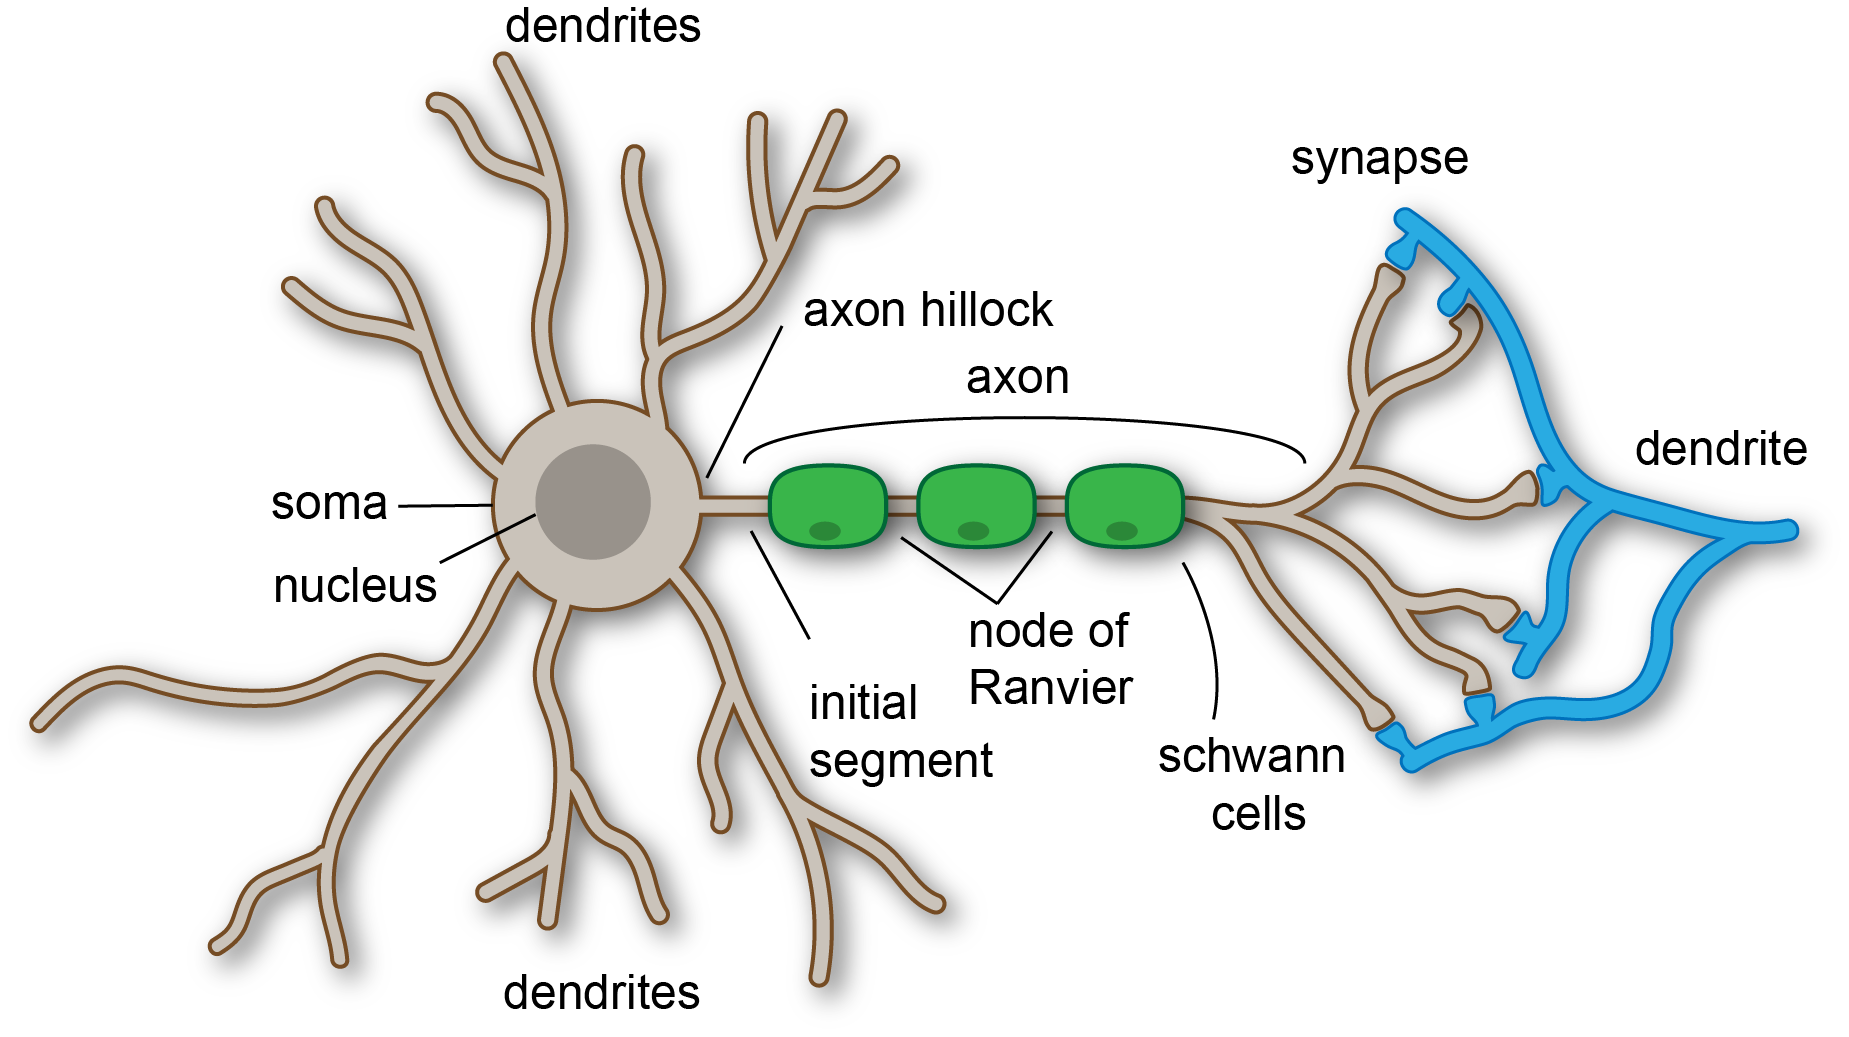
\includegraphics[width=\textwidth]{anatomy_of_neuron.png}
                    \caption{\centering Anatomy of a neuron (\cite{anatomy_of_neuron:2022})}
                    \label{fig:anatomy-of-neuron}
                \end{subfigure}
                \hfill
                \begin{subfigure}[b]{0.49\textwidth}
                    \centering
                    \resizebox{\textwidth}{!}{
                        \begin{tikzpicture}[
                            neuron/.style={rectangle, draw=dark_grey, rounded corners, minimum width=2cm, minimum height=1.5cm, thick},
                            input/.style={circle, draw=dark_grey, fill=light_grey, minimum size=0.8cm, thick},
                            output/.style={rectangle, draw=dark_grey, fill=light_grey, minimum size=0.8cm, thick},
                            node distance=0.5cm and 3cm,
                            >=latex,
                            transform shape
                        ]
                            % nodes
                            \node[input] (x1) at (0,0){$x_1$};
                            \node[input] (x2) [below=of x1]{$x_2$};
                            \node[input] (x3) [below=of x2]{$x_3$};
                            \node (dots) [below=0.5cm of x3] {$\vdots$};
                            \node[input] (xn) [below=of dots]{$x_n$};
                            \node[neuron] (neuron) [right=of x3] {neuron's soma};
                            \node[output] (output) [right=2cm of neuron] {axon};

                            % connections
                            \draw[->] (neuron) -- (output);
                            \foreach \i in {1,2,3,n} {
                                \draw[->] (x\i) -- (neuron)
                                    node[pos=0.5, sloped, above]{$w_\i$};
                            }
                        \end{tikzpicture}
                    }
                    \caption{\centering Schematic anatomy of a neuron (Adapted from: \cite{Aggarwal:2018})}
                    \label{fig:schematic-anatomy-of-neuron}
                \end{subfigure}
                \caption{\centering Detailed and schematic anatomy of a neuron}
            \end{figure}

            The artificial neuron is a basic processing unit and a building block of artificial neural networks (\cite{Alpaydin:2014}). At the same time, single artificial neuron builds a single-layer neural network. Single-layer networks may also include several artificial neurons in parallel. Layers of artificial neurons build complex neural networks that are also referred to as multilayer neural networks. Neural networks use representation learning (\cite{LeCun:2015}). This means that the artificial neural network discover the patterns in the data automatically without preprocessing the raw data (\cite{LeCun:2015}). The neural networks learn different representations of the input data at each of the layers (\cite{LeCun:2015}). The preprocessing of the raw data to extract important features has to be done in some conventional machine-learning approaches such as K-Nearest Neighbors technique.

            The following paragraphs will describe and provide insights into the single-layer and multilayer neural networks.

            \paragraph{Single-layer Neural Networks}
            \label{par:single-layer-neural-networks}
                \autoref{fig:artificial-neuron} describes the structure of an artificial neuron. The input values of an artificial neuron define a vector $\mathbf{x} = [x_1 \cdots x_N]^T$, where $x_j \in \mathbb{R}$ and $j \in \{1, \cdots, N\}$ (\cite{Alpaydin:2014}). The $N$ describes the total number of input values of an artificial neuron. The associated weights for each of the input values also define a vector $\mathbf{w_i} = [w_{i,1} \cdots w_{i,N}]^T$, where $w_{i,k} \in \mathbb{R}$, $k \in \{1, \cdots, N\}$ (\cite{Alpaydin:2014}). The $i$ denotes the index of an artificial neuron within the single-layer neural network. The bias $b_i$ is used to make the computation of an artificial neuron more general (\cite{Alpaydin:2014}). It adds fixed offset to the input of the artificial neuron (\cite{Bishop:2024}). We can add the bias to the $\mathbf{x}$ and $\mathbf{w_i}$ vectors. We obtain the extended vectors $\mathbf{x} = [1, x_1 \cdots x_N]^T$ and $\mathbf{w_i} = [b_i, w_{i,1} \cdots w_{i,N}]^T$. The artificial neuron performs the dot product of the vectors $\mathbf{w_i}^T$ and $\mathbf{x}$ (\cite{Alpaydin:2014}). The dot product of the vectors as matrix multiplication is defined as:
                \begin{equation}
                    \mathbf{w_i}^T\mathbf{x} = \sum_{n=1}^{N+1} w_{i,n} x_n = w_{i,1} + w_{i,2}x_2 + w_{i,3}x_3 + \cdots + w_{i,N+1} x_{N+1}.
                    \label{eq:dot-product-complex}
                \end{equation}
                In \autoref{eq:dot-product-complex}, the summand $w_{i,1}$ equals to $b_i$. We can reflect this and modify the \autoref{eq:dot-product-complex}. We get the following modified equation:
                \begin{equation}
                    \mathbf{w_i}^T\mathbf{x} = \sum_{n=2}^{N+1} w_{i,n} x_n + b_i.
                    \label{eq:dot-product-complex-modified}
                \end{equation}
                In \autoref{fig:artificial-neuron}, the symbol $\sum$ represents the summation operation that computes the dot product of the input vector and its associated weight vector as matrix multiplication. Further, the artificial neuron applies an activation function to the result of the dot product. This operation is defined as:
                \begin{equation}
                    y_{a_{i}} = f(\mathbf{w_i}^T\mathbf{x}).
                    \label{eq:activation-function-complex}
                \end{equation}
                The result of \autoref{eq:activation-function-complex} denoted as $y_{a_{i}}$ represents the output value of the artificial neuron with the index $i$ within the layer $l$.The activation function is denoted as $f$ in \autoref{fig:artificial-neuron}.

                \begin{figure}[h]
                    \centering
                    \begin{tikzpicture}[
                        input/.style={draw=dark_blue, fill=light_blue, thick, minimum size=0.8cm},
                        neuron/.style={circle, draw=dark_green, fill=light_green, minimum size=1cm, thick},
                        output/.style={draw=dark_red, fill=light_red, thick, minimum size=0.8cm},
                        node distance=0.8cm and 3cm,
                        >=latex,
                    ]
                        \coordinate (top) at (0,2);

                        %nodes
                        \node[input] (x1) at (0,0){$x_1$};
                        \node[input] (x2) [below=of x1]{$x_2$};
                        \node[input] (x3) [below=of x2]{$x_3$};
                        \node (dots) [below=0.5cm of x3] {$\vdots$};
                        \node[input] (xn) [below=of dots]{$x_n$};
                        \node[neuron] (artificial_neuron) [right=of x3]{$\sum$ \hspace{0.5em} $f$};
                        \draw[thick, draw=dark_green] (artificial_neuron.north) -- (artificial_neuron.south); % artificial neuron
                        \node[above=0.2em of artificial_neuron] {$a_{i}$}; % artificial neuron
                        \node (bias) at (artificial_neuron |- xn) {$1$};
                        \node[output] (output) [right=of artificial_neuron] {$y_{a_{i}}$};

                        % labels
                        \node[dark_blue] (inputs_label) at (x1 |- top) {Inputs};
                        \node[dark_green] (artificial_neuron_label) at (artificial_neuron |- top) {Artificial neuron};
                        \node[dark_red] (output_label) at (output |- top) {Output};

                        % connections
                        \foreach \m in {1,2,3,n} {
                            \draw[->] (x\m) -- (artificial_neuron)
                                node[pos=0.4, sloped, above] {$w_{i,\m}$};
                        }
                        \draw[->] (artificial_neuron) -- (output);
                        \draw[->] (bias) -- (artificial_neuron) node[midway, left] {$b_i$};
                    \end{tikzpicture}
                    \caption{\centering Artificial neuron (Adapted from: \cite{Aggarwal:2018})}
                    \label{fig:artificial-neuron}
                \end{figure}

                Artificial neurons may use different activation functions depending on the task they should accomplish (\cite{Aggarwal:2018}). In the following examples of activation functions I will denote the dot product from \autoref{eq:dot-product-complex-modified} simply as $x$. The most basic activation function is the identity function (\cite{Aggarwal:2018}):
                \begin{equation}
                    f(x)=x.
                    \label{eq:identity-function}
                \end{equation}
                Other activation functions are (\cite{Aggarwal:2018}): the sign function
                \begin{equation}
                    f(x)=\text{sign}(x),
                    \label{eq:sign-function}
                \end{equation}
                the sigmoid function
                \begin{equation}
                    f(x) = \frac{1}{1 + e^{-x}},
                    \label{eq:sigmoid-function}
                \end{equation}
                the hyperbolic tangent function (tanh)
                \begin{equation}
                     f(x) = \frac{e^{2x}-1}{e^{2x}+1},
                    \label{eq:tanh-function}
                \end{equation}
                and the rectified linear unit function (ReLU)
                \begin{equation}
                    f(x) = \max(0, x).
                    \label{eq:relu-function}
                \end{equation}
                The sign activation function divides the input space into two half-spaces where its output is either positive or negative (\cite{Alpaydin:2014}). This function outputs either $1$ or $-1$. A single artificial neuron using the sign$(x)$ activation function, also called perceptron, can be used for binary classification (\cite{Aggarwal:2018}). While a perceptron with only one input defines a line, a perceptron with two inputs defines a plane and a perceptron with more than two inputs defines a hyperplane (\cite{Alpaydin:2014}). The sigmoid activation function, whose output values are from the interval $(0,1)$, is used when the output of an artificial neuron is interpreted as a probability. The tanh activation function outputs values from the interval $[-1,1]$ and the ReLU from the interval $[0, \infty)$. The sigmoid, tanh and ReLU activation functions are particularly applied in multilayer neural networks (\cite{Alpaydin:2014}). The sigmoid and tanh activation functions are saturating functions (\cite{Murphy:2022}). This means that for large positive numbers the sigmoid activation function outputs values approaching $1$. The tanh activation function outputs $1$. For large negative numbers, the sigmoid activation function outputs values approaching $0$ and the tanh activation function outputs $-1$.

                To build and train a single-layer neural network, we have to define not only the activation but also the loss function for the artificial neurons. In supervised learning, the loss function quantifies the difference, or loss, between the expected value and the real output of the artificial neuron (\cite{Mohri:2018}). In term of unsupervised learning, the loss function measures the difference between the predicted output and original input of the neural network (\cite{Bishop:2024}). The concept of unsupervised learning becomes significant in multilayer neural networks. The \autoref{tab:single-layer-single-neuron-models} shows examples of different single-layer neural networks consisting of single artificial neuron and the activation and loss functions used in these models. The loss function represents the loss of the neuron for the training sample with the index $t$. The $y_t$ stands for the prediction and $\hat{y}_t$ for the label of the training pair.
                \begin{table}[h]
                    \centering
                    \begin{tabular}{|c|c|c|}
                        \hline
                        model & activation function & loss function\\
                        \hline
                        perceptron with discrete output & sign function &  $\mathcal{L}_{t}(y_i, \hat{y}_t) = (y_t - sign(\hat{y}_t))^2$ \\
                        perceptron with continuous output & identity function & $\mathcal{L}_{t}(y_t, \hat{y}_t) = \max(0, -y_t \cdot \hat{y}_t)$ \\
                        linear regression & identity function & $\mathcal{L}_{t}(y_t, \hat{y}_t) = (y_t - \hat{y}_t)^2$ \\
                        logistic regression  & sigmoid function & $\mathcal{L}_{t}(y_t, \hat{y}_t) = -\text{log}(\abs{\frac{y_t}{2} -0.5 + \hat{y}_t})$ \\
                        support vector machine (SVM)& identity function & $\mathcal{L}_{t}(y_t, \hat{y}_t) = \max(0, -y_t \cdot \hat{y}_t + 1)$  \\
                        \hline
                    \end{tabular}
                    \caption{\centering Single-layer neural network models consisting of a single artificial neuron (Adapted from: \cite{Aggarwal:2018})}
                    \label{tab:single-layer-single-neuron-models}
                \end{table}
                Perceptron with discrete output and support vector machine models may be used for binary classification (\cite{Alpaydin:2014}). Both of the models output real values. Logistic regression model may be used for the same task by predicting the probability for a positive class (\cite{Aggarwal:2018}). Linear regression model and perceptron with continuous output may be used for predicting a real-valued label of a problem instance represented as an input vector (\cite{Bishop:2024}).

                Increasing the number of artificial neurons in a single-layer network, we extend the capabilities of a single-layer neural network. The \autoref{tab:single-layer-multiple-neuron-models} shows examples of different single-layer neural networks consisting of more than one artificial neuron. The table also shows the activation and loss function of the artificial neurons.
                \begin{table}[h]
                    \centering
                    \begin{tabular}{|c|c|c|}
                        \hline
                        model & activation function & loss function \\
                        \hline
                        multiclass perceptron & identity function &  $\mathcal{L}_{t}(\mathbf{\hat{y}}) = \max_{i:i \neq c(t)}\max(\hat{y}_i - \hat{y}_{c(t)}, 0)$ \\
                        multiclass SVM & identity function & $\mathcal{L}_{t}(\mathbf{\hat{y}}) = \sum_{i:i \neq c(t)}\max(\hat{y}_i - \hat{y}_{c(t)} + 1, 0)$ \\
                        multinomial logistic regression & softmax function & $\mathcal{L}_{t}(\mathbf{\hat{y}}) = -log(-\hat{y}_{c(t)})$ \\
                        \hline
                    \end{tabular}
                    \caption{\centering Single-layer neural network models consisting of multiple artificial neurons (Adapted from: \cite{Aggarwal:2018})}
                    \label{tab:single-layer-multiple-neuron-models}
                \end{table}
                All of the three models in \autoref{tab:single-layer-multiple-neuron-models} are used for multiclass classification problems. Each artificial neuron represents single class or label from the training set. The multiclass perceptron models as well as multiclass support vector machine models return real values (\cite{Aggarwal:2018}). The multinomial logistic regression models return probabilities for each of the classes represented by the neurons in the single-layer neural network. In addition, multinomial logistic regression models use the softmax activation function:
                \begin{equation}
                    y_{a_{i}}^t = \frac{e^{\mathbf{w_i}^T\mathbf{x}^t}}{\sum_{j=1}^{n} \mathbf{w_k}^T\mathbf{x}^t}.
                    \label{eq:softmax-function}
                \end{equation}

                In \autoref{tab:single-layer-multiple-neuron-models}, the index $c(t)$ represents the index of an artificial neuron representing the true class for the training pair with index $t$. The loss function of a multiclass single-layer neural network compares the actual output of a neuron with the output of the neuron that represents the true class. The loss function of a multiclass support vector machine computes the maximum between $\hat{y}_i - \hat{y}_{c(t)} + 1$ and $0$ for each neuron representing a class that is different from the true class. The maximum values are then summed to a single loss value.

                The general rule for updating the weights of the weight vector $\mathbf{w_i}$ of an artificial neuron $a_{i}$ within a single-layer neural network can be defined as (\cite{Aggarwal:2018}):
                \begin{equation}
                    \mathbf{w_i} = \mathbf{w_i} - \alpha \cdot \frac{\partial \mathcal{L}_t}{\partial \mathbf{w_i}}.
                    \label{eq:gradient}
                \end{equation}
                The scaling factor $\alpha$ is called the learning rate (\cite{Aggarwal:2018}). The partial difference $\frac{\partial \mathcal{L}_t}{\partial \mathbf{w_i}}$ of loss function $\mathcal{L}_t$ with respect to the weights $\mathbf{w_i}$ is also called the gradient. That is why this update technique is called gradient descent. The \autoref{eq:gradient} assumes that the loss function is differentiable (\cite{Aggarwal:2018}).

                % stochastic gradient descent as optimization
                The limitation of the single-layer neural network is that they only learn or are limited by linear boundaries of the input space regardless of the activation function (\cite{Bishop:2024}). For example, the output values in single-layer classification can classify only data that are linearly separable (\cite{Bishop:2024}). This means that the data input space must be linearly separable by lines, planes or hyperplanes, depending on its dimensionality (\cite{Bishop:2024}).

            \paragraph{Multilayer Neural Networks}
            \label{par:multilayer-neural-networks}

                Multilayer neural networks contain more than one computational layer of artificial neurons. Typically, multilayer neural networks have input, output and multiple hidden layers. In \autoref{par:single-layer-neural-networks}, I have briefly described the limitations of single-layer neural networks. These are not limitations for multilayer neural networks. The multilayer neural networks can learn more complex patterns in the data by transforming the input space in a way that makes the data in the input space linearly separable (\cite{LeCun:2015}). This ability of neural networks is achieved by the hidden layers. More formally, the power of multilayer neural networks to explore non-linear patterns in the data comes from the repeated composition of non-linear functions over multiple layers of the network (\cite{Aggarwal:2018}). This increases the representational power of a multilayer neural network and lowers the numbers of parameters of the network (\cite{Aggarwal:2018}). Each layer of a multilayer neural network learns different representations of the input space (\cite{LeCun:2015}). The representations are obtained by combining simple representations at lower layer into abstract representations at higher layers. Through this composition of different representations very complex functions may be learned by the neural networks (\cite{Bishop:2024}). Thus, multilayer neural network are able to explore complex patterns in high-dimensional input data (\cite{LeCun:2015}). An example would be a neural network learning to classify different objects. At lower layers, the neural network learns the presence of horizontal and vertical lines. At the higher levels, these representations are combined into abstract features of the objects such as edges or textures. This enables the neural networks to learn the distinguishing features of the objects and correctly classify them.

                Neural networks with a few hidden layers are considered shallow. Multilayer neural networks with many hidden layers are considered deep. Deep neural networks are at the forefront of neural networks research (\cite{LeCun:2015}). Nowadays, when discussing multilayer neural networks, a deep architecture with many layers is meant usually. The subfield of machine learning that deals with deep neural networks is called deep learning. At the core of deep learning, there is the representation learning (\cite{LeCun:2015}). As stated previously, it enables the deep neural networks to learn different abstractions of the input data at each of the layers by combining simple representations to get abstract representations of the input data (\cite{LeCun:2015}). The representation learning also allows to use the unlabeled data because it forces the neural network to explore structures in the data (\cite{Bishop:2024}).

                A standard deep multilayer architecture of a neural network is a stack of many layers of artificial neurons (\cite{LeCun:2015}). Deep neural networks learn a non-linear mapping from a fixed-dimensional input to a fixed-dimensional output (\cite{LeCun:2015}). Information flows in a feed-forward way from the input layer, thought the hidden layers, to the output layer. At each layer of a deep neural network, artificial neurons compute the weighted sum of the inputs from the previous layer. Artificial neurons apply then a non-linear activation function to the weighted sum and forward the result to the next layer. The most common non-linear function used in deep neural networks is the rectified linear unit (ReLU) activation function described in \autoref{par:single-layer-neural-networks}. The convolutional neural networks (CNNs) and the recurrent neural networks (RNNs) are examples of deep neural networks. These types of neural networks are used for sequential data such as sentences or time-series (\cite{Aggarwal:2018}). Convolutional neural networks are discussed in greater detail in \autoref{subsub:convolutional-neural-networks}.

                Deep neural networks are trained using the process of backpropagation. The backpropagation algorithm adjusts the incoming weights of artificial neurons at every layer of the neural network. As mentioned in the \autoref{par:single-layer-neural-networks}, the adjustment of weights or parameters in a single-layer neural network is relatively easy. The problem in multilayer neural network is that the loss computed using a loss function at the output layer is also affected by the parameters in the previous layers. It is not sufficient to adjust the incoming weights of artificial neurons only at the output layer. The loss has to be propagated backwards to the previous layers of the neural network. The loss function is applied to an output that is a result of a composition of functions from the previous layers (\cite{Bishop:2024}). The contribution of any parameter within the neural network is the partial derivative of the loss function with respect to the parameter (\cite{Bishop:2024}). The backpropagation algorithm has to apply the chain rule to compute this contribution (\cite{Aggarwal:2018}). The parameters within the neural network will be then adjusted by their contribution and a learning factor in the same way as those in the single-layer neural networks.

                When training a deep neural network, several issues and problems may arise. One of them is the problem of overfitting. When a neural network suffers from overfitting, it is very accurate on the training dataset but generalizes poorly on new, unseen data (\cite{Aggarwal:2018}). The overfitting problem is a consequence of the bias--variance tradeoff (\cite{Aggarwal:2018}). By increasing the number of trainable parameters in a model, it becomes more powerful in learning from the training dataset (\cite{Aggarwal:2018}). This means that the model becomes less biased (\cite{Aggarwal:2018}). Training deep neural networks with a high number of parameters on different limited subsets of a larger dataset would produce high variance of predictions when the models are tested on the same dataset (\cite{Aggarwal:2018}). It is important to choose the optimum between the complexity of a model and the size of a dataset (\cite{Aggarwal:2018}). To minimize overfitting, regularization methods may be used (\cite{Aggarwal:2018}). Regularization methods are used to reduce the representational capacity of a model (\cite{Goodfellow:2016}). There are different regularization methods, for example: weight decay, dropout, or early stopping. The weight decay method adds a penalty term to the loss function (\cite{Bishop:2024}). This method makes the parameters or weights of a deep neural network decay towards zero (\cite{Bishop:2024}). It prevents a deep neural network from learning high weight values (\cite{Bishop:2024}). The dropout method excludes a neuron and all its incoming or outgoing connections from the learning process (\cite{Aggarwal:2018}). A neuron is typically excluded with a probability between 20\% and 50\% (\cite{Aggarwal:2018}). This way, one or many different neural networks may be created from a base network and trained using shared parameters (\cite{Aggarwal:2018}). The early stopping method stops the execution of the backpropagation algorithm when the loss of the networks starts to rise on the validation dataset (\cite{Murphy:2022}).

                The next problem is the vanishing and exploding gradients. When training a deep neural network, the behavior of saturating functions such as sigmoid or tanh creates the vanishing gradient problem (\cite{Murphy:2022}). In the saturated regions of these saturating functions, the gradient of the output of the function with respect to the function's input approaches $0$ (\cite{Murphy:2022}). The vanishing gradient problem can be solved using the ReLU activation function. Activation functions that have expected values higher than $1$ cause the exploding gradient problem (\cite{Aggarwal:2018}). To minimize the exploding and vanishing gradient problem, batch normalization is used (\cite{Aggarwal:2018}). Batch normalization normalizes the output values to have a mean of zero and a unit variance after each mini-batch consisting of a specific number of training samples (\cite{Szegedy:2015:2}). Batch normalization also solves the problem of the internal covariate shift (\cite{Aggarwal:2018}). The internal covariate shift describes a change of distribution of output values in a neural network (\cite{Szegedy:2015:2}). The output values change because of the change in the network parameters during the training process (\cite{Szegedy:2015:2}).

                There are also several optimization strategies for gradient descent applied to optimize the learning process of a deep neural network. The standard gradient descent refers to the batch gradient descent (\cite{Li:2022}). In this method, the gradient of the loss function is computed over the whole training dataset (\cite{Gu:2018}). One of the optimizations to the standard gradient descent is the stochastic gradient descent. This optimization computes the gradient after each training sample (\cite{Li:2022}). The mini-batch gradient descent optimization computes the gradient after a small part of training samples in order to be more efficient as the batch gradient descent optimization (\cite{Li:2022}). There are several other gradient descent optimizations. The momentum algorithm uses the exponentially weighted average of the gradients to update network's parameters (\cite{Li:2022}). The AdaGrad optimization algorithm keeps an aggregated squared partial derivative with respect to each network's parameter (\cite{Aggarwal:2018}). During every algorithm iteration, the aggregated value for each parameter is updated. Next, the computed gradient is scaled by the fraction of learning rate and the root of the aggregated squared gradients (\cite{Aggarwal:2018}). The RMSProp algorithm uses exponentially averaged squared partial derivatives with respect to each network's parameter (\cite{Aggarwal:2018}). The update of the parameters is the same as in the AdaGrad algorithm. The Adam algorithm uses two exponentially averaged squared partial derivative values with respect to each network's parameter, but computed with different decay parameters (\cite{Aggarwal:2018}). The update of each parameter is computed as the multiplication of the fraction of the learning rate and the root of the first exponentially aggregated squared gradient and the second exponentially aggregated squared gradient (\cite{Aggarwal:2018}).

        \subsubsection{Convolutional Neural Networks (CNNs)}
        \label{subsub:convolutional-neural-networks}

        Convolutional neural networks are based on the cat's visual cortex (\cite{Aggarwal:2018}). The visual cortes is a part of the brain responsible for processing visual information. Researchers studying visual cortex of cats discovered that different parts of the visual cortex are sensitive to different elements or features of the visual field (\cite{Aggarwal:2018}). The visual cortex of a cat has a layered structure (\cite{Aggarwal:2018}). Layers of biological neurons are stacked upon each other to extract different features and elements of the visual field (\cite{Aggarwal:2018}). For example, when a cat perceives a square object, a different group of cells in the visual cortex is excited than when it perceives a round object (\cite{Aggarwal:2018}).

        The layered structure of the cat's visual cortex with its feature extraction ability by different visual cortex regions was the primary inspiration to develop convolutional neural networks. From the machine learning perspective, the cat's visual cortex hierarchically extracts and combines simpler abstractions of the visual input into more complex ones (\cite{Aggarwal:2018}). This way, the visual cortex extracts complex features of the visual field, for example objects in the visual input (\cite{Aggarwal:2018}). Convolutional neural networks achieve similar hierarchical feature extraction by combining primitive shapes like horizontal lines from earlier layers into complex features at later layers (\cite{Aggarwal:2018}). Convolutional neural networks work on grid-structured input data (\cite{Aggarwal:2018}). Grid-structured input data such as images contain spatial dependencies (\cite{Aggarwal:2018}). The pixels in close proximity have highly correlated values (\cite{Bishop:2024}). In case of images, the spatial dependencies are, for example: horizontal and vertical lines, edges, textures, and objects. To simulate the activation of different regions of cat's visual cortex, convolutional neural networks detect the spatial dependencies of the input data by applying the convolution operation (\cite{Aggarwal:2018}). A convolution operation uses various grid-structured filters to extract different features from a grid-structured input data or its abstractions at later layers of a network (\cite{Aggarwal:2018}).

        All the training issues, normalization and regularization methods, and optimizations of the gradient descent presented in \autoref{par:multilayer-neural-networks} apply naturally to CNNs.

            \paragraph{Architecture of a CNN for Image Classification}

                A convolutional neural network follows the traditional feed-forward structure of a standard deep neural network, except that the feature extraction operations in the layers of a network are spatially organized (\cite{Aggarwal:2018}). This means that these operations process only small regions of the output from the previous layers (\cite{Aggarwal:2018}). Moreover, the spatial organization results in sparse connections and spatial relationships between layers, as each operation connects only to a local region of the previous layer (\cite{Aggarwal:2018}). Convolutional neural networks are built using three types of layers: convolutional, pooling and ReLU layers (\cite{Aggarwal:2018}). Final layers of a convolutional neural network are usually fully connected layers (\cite{Aggarwal:2018}). A ReLU layer usually follows a convolutional layer, applying non-linear activation to the output of a convolution operation (\cite{Aggarwal:2018}). After multiple pairs of convolutional and ReLU layers, a pooling layer is used (\cite{Aggarwal:2018}).

                As stated previously, convolutional neural networks process grid-structured data. The input data has not only spatial dimensions (width and height) but also depth. For example, a color picture has width and height and three color channels. The output of convolutional layers or pooling layers also has a three-dimensional structure. The depth of an output consists of various layers of features extracted from the input (\cite{Aggarwal:2018}). Convolutional layers apply kernels or filters to their inputs (\cite{Aggarwal:2018}). A filter is a three-dimensional structural unit containing real values as parameters (\cite{Aggarwal:2018}). Spatial dimensionality of a filter is smaller than the spatial dimensionality of its input (\cite{Aggarwal:2018}). On the other hand, a filter has the same depth as its input (\cite{Aggarwal:2018}). A convolutional layer may contain several of these filters. All filters have the same spatial dimensionality and depth. The number of filters used by a convolutional layer gives the depth of the layer's output (\cite{Aggarwal:2018}). Usually, the width and height dimensions of filters or inputs are also equal (\cite{Aggarwal:2018}). For example, an input may have the size $16 \times 16 \times 5$ and a filter may have spatial dimensions of $3 \times 3$ and a matching depth of $5$.

                Let's assume that an input of a convolutional layer with index $q$ is of dimensions $I_{q} \times I_{q} \times d_q$. This layer uses $N$ different filters of dimensions $F_{q} \times F_{q} \times d_q$. The convolutional operation places the filter at all possible spatial positions and performs dot product between the region of the input and the filter (\cite{Aggarwal:2018}). The input region and the filter are treated as vectors with the size $F_{q} \times F_{q} \times d_q$. Applying a filter to the input of a layer results in a feature map (\cite{Aggarwal:2018}). The resulting width and height of the layer's output are computed as $O_{q} = I_{q} - F_{q} + 1$. This represents the number of different placements of the filter in the horizontal or vertical axis of the input grid. The filter does not exceed the input grid boundaries. The resulting output of the layer is of dimensions $O_{q} \times O_{q} \times d_N$. Convolution operation reduces spatial dimensionality of the output when compared to the input. To not lose the information around the borders of the input grid, padding is used (\cite{Aggarwal:2018}). To reduce the level of granularity of the convolution operation, the stride of a filter is used (\cite{Aggarwal:2018}). Commonly, the stride is of value $1$ (\cite{Aggarwal:2018}). This means that a filter moves by one grid cell along both horizontal and vertical axes. By increasing the stride value, a filter will move by that number of cells along the spatial dimensions.

                For all $O_{q} \times O_{q} \times d_N$ output values of a convolutional layer, the ReLU activation function is applied. Applying the ReLU activation function to the input does not change its dimensionality (\cite{Aggarwal:2018}). The pooling layer performs operations on small regions of size $P_{q} \times P_{q}$ on all $d_{q}$ feature maps of an input (\cite{Aggarwal:2018}). The pooling operation goes through all the possible regions of $P_{q} \times P_{q}$ size in a feature map and selects the maximum value from a region that is in focus. This is also called the max-pooling. The notion of stride also applies in a pooling operation (\cite{Aggarwal:2018}). The stride defines where the next region that the max-pooling will be performed on is located. Pooling layer does not change the depth of the input because the pooling operations are performed on all its feature maps (\cite{Aggarwal:2018}). However, pooling layer significantly changes the spatial dimensionality of the input (\cite{Aggarwal:2018}). For example, performing a pooling operation with a region size of $2 \times 2$ with stride of $2$ on a single feature map of size $4 \times 4$ reduces the spatial dimensionality of the output to $2 \times 2$.

                The layers at the end of a CNN are fully connected layers as in a standard feed-forward deep neural network (\cite{Aggarwal:2018}). There may be more than one fully connected layer used. All the parameters of the last convolutional--activation layer pair or of the last pooling layer are connected with all the neurons in the first fully connected layer (\cite{Aggarwal:2018}). The activation function used in the last layer depends on the task a CNN is trained for (\cite{Aggarwal:2018}). For a classification task, the softmax activation function is used.

                There are different CNN architectures for image classification: AlexNet, VGGNet, ResNet, GoogLeNet, Inception (following iterations of GoogLeNet), DenseNet, ResNeXt, Xception, MobileNet, GhostNet, EfficientNet, or EfficientNetV2. There are also different variants of these architectures differing mainly in the depth of the networks, such as DenseNet-121, DenseNet-201, ResNet-50, ResNet-101, Inception v2, or Inception v3. \autoref{fig:lenet5-architecture} shows the LeNet-5 architecture created by \textcite{LeCun:1998}. It was an early approach to CNNs. The LeNet-5 architecture has three convolutional layers, two pooling or subsampling layers and two fully connected layers. The architecture uses the tanh activation function.
                \begin{figure}[h]
                    \centering
                    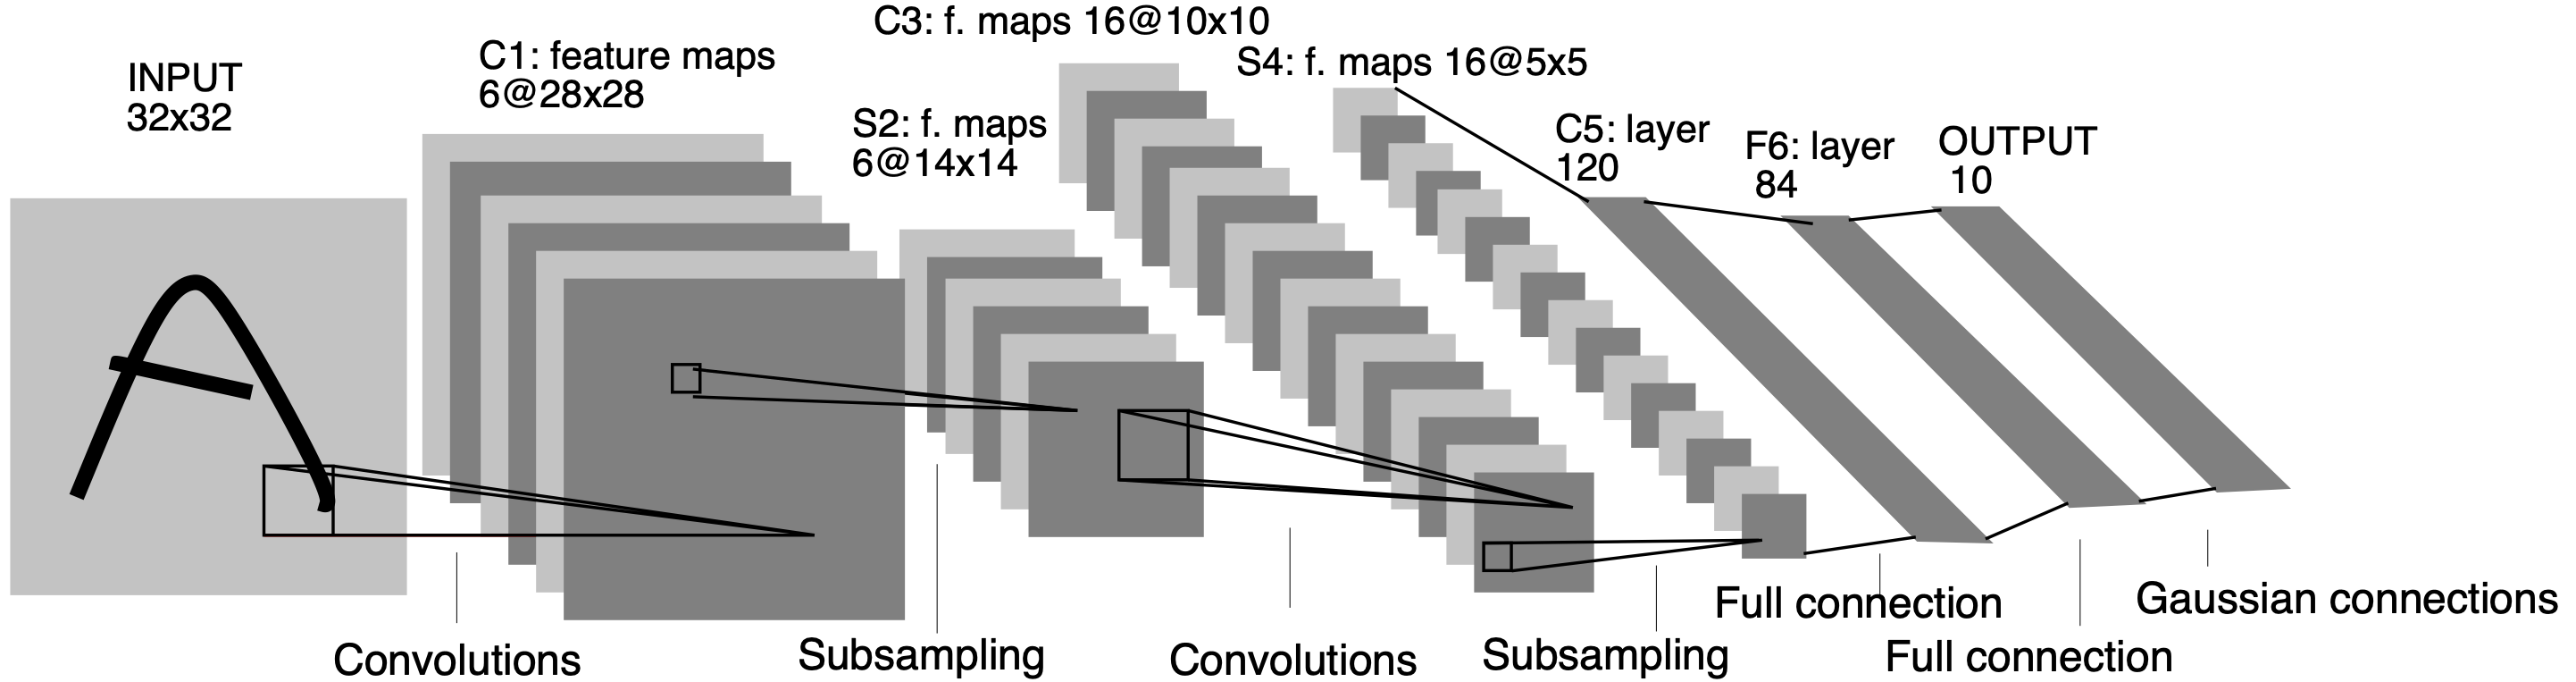
\includegraphics[width=\textwidth]{lenet5_architecture.png}
                    \caption{\centering LeNet-5 architecture (Source: \cite{LeCun:1998})}
                    \label{fig:lenet5-architecture}
                \end{figure}

    \subsection{Related Research}

        \textcite{Sladojevic:2016} used a new machine learning method to recognize and classify plant diseases from leaf images. The authors used a convolutional neural network. The development in deep learning algorithms and GPUs enabled the authors to train and test a CNN model on a normal computer. \textcite{Sladojevic:2016} trained a CaffeNet model to recognize 15 different classes of images. Out of these 15 classes, 13 classes were plant--disease pairs, one class was used for healthy images, and one for images with background. \textcite{Sladojevic:2016} created the initial dataset by collecting the images from the Internet. The authors then resized the collected images to $256 \times 256$ to reduce the training time. Furthermore, the authors increased the robustness of the initial dataset by augmenting the images. Augmenting the dataset also reduces overfitting of a model during the training process. The authors applied affine and perspective transformation, and simple rotations. The final dataset contained almost 34,000 images. The number of images in individual classes varied. The CaffeNet model was pre-trained on the ImageNet dataset outputting the probabilities for 1,000 image classes. This is why the authors modified the CaffeNet architecture to output the probabilities for each of the 15 classes. To validate the model's performance, the authors used the 10-fold cross validation technique. A model trained using transfer learning without the fine-tuning step reached an overall accuracy of 95.8\%. A model trained using the fine-tuning step reached an overall accuracy of 96.3\%. \textcite{Sladojevic:2016} noted that the fine-tuning step during the training did not increase the accuracies of the trained models significantly. On the other hand, both trained models reported higher accuracies in classes with a higher number of images.

        \textcite{Mohanty:2016} trained two CNN architectures, GoogLeNet and AlexNet, from scratch and using transfer learning with fine-tuning on the PlantVillage dataset. This dataset was published by \textcite{Hughes:2015}. The models trained using transfer learning were pre-trained on the ImageNet dataset. The PlantVillage dataset contained 54,306 images divided into 38 classes of plant--disease pairs. In this research, the authors used three different versions of the PlantVillage dataset: the original color version, a grey-scale version, and a segmented version. In the segmented version of the dataset, the authors removed the background and left only the leaf surface. The authors resized all images to $256 \times 256$ pixels. Further, the authors used five different train--test split ratios of the dataset: 80\% of the dataset for training and 20\% for testing, 60\% of the dataset for training and 40\% for testing, 50\% of the dataset for training and 50\% for testing, 40\% of the dataset for training and 60\% for testing, and finally 20\% of the dataset for training and 80\% for testing. In total, the authors created 60 different experiment settings having two different training strategies, two different CNN architectures, three dataset versions, and five different train--test split ratios of these three datasets. Prior to the training process, the authors modified the final layer of all models to output 32 probabilities for all the classes in the dataset.

        The overall accuracies over all the experiment settings varied from 85.53\% to 99.43\%. The accuracy at the low interval border was achieved by an AlexNet model trained from scratch using 80\% of the gray-scale dataset version for training and the remaining part for testing. The accuracy on the interval border was achieved by a GoogLeNet model trained using transfer learning method. In this case, 80\% of the dataset were used for training and the remaining 20\% of the dataset were used for testing. The authors stated that the overall accuracy of the models decreases when the train subset to test subset ratio is increased. Furthermore, the authors stated that among all trained models, models with GoogLeNet architecture achieved higher average accuracies than those with AlexNet architecture. Also, models trained using transfer learning method performed better than those trained from scratch. Among all three dataset versions, models trained on the color version of the PlantVillage dataset outperformed all other models. Moreover, models trained using transfer learning method with the fine-tuning step converged after significantly lower number of epochs than models trained from scratch. An epoch describes a full pass through the training dataset.

        The authors also validated the performance of the model with the highest achieved average accuracy on two datasets containing images from other sources. The model achieved an average accuracy of 31.40\% and 31.69\% on these datasets. This inability of the model to generalize on different images was caused by the lack of variability of images in the PlantVillage dataset. The authors of the PlantVillage dataset took the images under controlled conditions. All images have neutral backgrounds and uniform lighting. Complex backgrounds containing other objects, different lighting conditions, and different leaf orientations in the images would increase the generalization ability of the models. Eventually, the authors stated that the models could not be used in practice, for example in a mobile application, at that point.

        \textcite{Ferentinos:2018} trained five different CNN architectures --- AlexNet, AlexNetOWTBn, GoogLeNet, Overfeat, and VGG --- on an extended PlantVillage dataset. The author did not state if the models were already pre-trained or were trained from scratch with random parameter values. The extended dataset contained 87,848 images and 58 classes of plant--disease pairs or healthy plants. \textcite{Ferentinos:2018} recognized the limited variability of the dataset used by \textcite{Mohanty:2016}. More than 1/3 of the images in the dataset used by \textcite{Ferentinos:2018} were taken under field conditions. These images had, for example, complex backgrounds containing irrelevant object or other plant parts and were taken under different lighting conditions. The author used 80\% of the dataset to train the models and remaining 20\% to test these models. In both training and testing subsets, the authors left the ratio between images taken under laboratory condition and images taken under field conditions the same as in the full dataset.

        Under this experiment setting, all five models achieved average accuracy of over 97\%. The best performing CNN models were AlexNetOWTBn with the average accuracy of 99.44\% and the VGG model with 99.48\%. Training the models using resized images to $256 \times 256$ pixels did not affect the average accuracy of the models. Using these two best performing models, the author investigated the impact of images taken under field conditions in the training dataset to the model performance. The author selected 12 classes from the initial dataset that either had only images taken under field or under laboratory conditions. The author then trained both of the best performing architectures on the images taken under field conditions and tested on images taken under laboratory conditions. Then, the author switched the training and testing subsets. As in (\cite{Mohanty:2016}), the average accuracy of the models decreased significantly. In the case of images taken under laboratory conditions used as a training dataset and images taken under field conditions as a testing dataset, the AlexNetOWTBn model achieved an average accuracy of 32.32\% and the VGG model an average accuracy of 33.27\%. In the reversed experiment setting, the AlexNetOWTBn model achieved an average accuracy of 62.57\% and the VGG model an average accuracy of 65.69\%. Images taken under field conditions indeed greatly impact the ability of a model to generalize on new images.

        All three experiment settings showed how the images in the training dataset impact model's ability to generalize. As in (\cite{Mohanty:2016}), this limited the use of the trained models in practice. Nevertheless, \textcite{Ferentinos:2018} stated that using a CNN model for classification of diseases from plant leaves is a promising approach. A robust training dataset is needed for a CNN model to generalize sufficiently well.

        % similar research papers with more modern approaches

        \textcite{Barbedo:2018:1} investigated the impact of datasets with limited size and variability on the accuracy of a CNN model to classify diseases from plant images. The author stated that datasets containing only images taken under laboratory conditions did not contain the symptom variety found under field conditions. The symptoms may also manifest on other plant parts than leaves. He also stated that the symptoms progress and change depending on several environmental factors, such as humidity and temperature. According to the author, the lack of variability in datasets not containing images taken under field conditions greatly influenced the generalizability of trained models. As an example, the author named the research by \textcite{Mohanty:2016}, where the accuracy of the models fell by 2/3 when tested on new unseen images. In (\cite{Mohanty:2016}), the models were trained using the PlantVillage dataset containing only images taken under controlled conditions.

        \textcite{Barbedo:2018:1} created a small dataset that contained a high variability of images. The dataset contained 1,383 images divided into 56 classes representing plant--disease pairs. The majority of images, about 85\%, were taken under field conditions. The rest was taken under controlled conditions. The number of images in each class varied from 5 to 77. When training a pre-trained GoogLeNet model, the author explicitly focused on the influence of background on the accuracy of the trained models. For this purpose, the author created a second version of the dataset containing images with removed background. The author removed the image backgrounds manually. Both dataset versions were augmented using affine transformations, random brightness increase and decrease, contrast enhancement and reduction, sharpness enhancement, and random Gaussian noise. The author used 80\% of the dataset for training and the remaining 20\% for testing. To obtain the final results, \textcite{Barbedo:2018:1} used the 10-fold cross validation method. The model trained on the original dataset achieved accuracies ranging from 65\% in case of wheat and common bean to 100\% in case of cotton. The model trained on the dataset containing images with removed background achieved accuracies ranging from 50\% in case of wheat to 100\% in case of cassava and sugarcane.

        The author then summarized the impact of background removal on the accuracies achieved by the model trained on the dataset containing images without background. Background removal had a positive effect in cases when the images had very busy backgrounds occupying a large portion of the images. The author observed a negative impact on image classes that had very similar symptom manifestation. This explains the decreased accuracy of the model in the case of wheat diseases. Very similar symptoms of wheat diseases led to the inability of the model to distinguish between them. For some crops, negative and positive effects were observed at the same time. \textcite{Barbedo:2018:1} observed no effect of background removal in the case of crops building at most three plant--disease classes and their diseases having distinctive symptom manifestations. The author noted that diseases that are rare or uncommon or have varied symptoms will always be classified with low accuracy.

        \textcite{Barbedo:2018:1} concluded that limiting the scope to only some small number of classes enables the collection of a very comprehensive dataset with a high variability of images.

        \textcite{Barbedo:2018:2} stated that many papers at that time, such as papers by \textcite{Mohanty:2016} or \textcite{Ferentinos:2018}, reported high accuracies of the trained models but these models were not applicable in the real world. Although reporting high accuracies on the training dataset, the model generalized poorly on unseen images. Like in (\cite{Barbedo:2018:1}), \textcite{Barbedo:2018:2} named the PlantVillage dataset as the main cause because it was not representative and robust enough. The author analyzed different factors influencing the performance of CNN models. These factors were: dataset of insufficient size and variety/variability, symptoms representation, covariate shift, image background, image capture conditions, symptom segmentation, symptom variations, multiple diseases on a single leaf, and diseases with similar symptoms.

        When analyzing the factors, \textcite{Barbedo:2018:2} summed up their impacts on the generalization ability of a trained model. Models trained on datasets containing very few images or having images with very busy backgrounds may rely more on the background information. Additionally, if certain objects or elements appear throughout the images in the dataset, these may disturb the learning process. Further, the absence of symptom variety or different development stages in the dataset weakens models' ability to generalize. Using the training and testing images from the same dataset leads to very high accuracies of the models. As shown by \textcite{Sladojevic:2016}, \textcite{Mohanty:2016}, and \textcite{Ferentinos:2018}, validating the performance of trained models on images from other sources than the original dataset leads to a significant decrease in accuracy. In order for a dataset to be representative, it has to contain images taken under various conditions. These conditions may include different lighting conditions, different weather conditions, different objects present, or different leaf orientations. Extending a dataset by segmenting the diseased regions of leaves increases models' ability to generalize. At different stages of a disease, the symptoms may have very different characteristics. A robust dataset has to include leaf images with diseases at different stages. In case of leaves that are diseased by various diseases, the solution is to segment each diseased region and label it accordingly. When diseases show similar symptom characteristics, a model relies heavily on background information. This may lead to high misclassification rates. The author did not present a solution to this problem.

        \textcite{Barbedo:2019} investigated the impact of images of individual diseased regions on model's classification accuracy. For this research, the author created a base dataset containing 1,567 images of plant leaves divided into 79 classes representing plant--disease pairs. Images in the dataset were captured under various conditions and included varied symptom characteristics for each class. About 60\% of the images in the dataset were taken under controlled conditions and the rest of the images was taken under field conditions. Further, the author created two other versions. One version contained only images of segmented leaf masks and the other version contained also images of segmented diseased regions. The dataset version including images of diseased regions contained 46,409 images. The author segmented the individual diseased leaf regions manually.

        \textcite{Barbedo:2019} used all three dataset versions to train a GoogLeNet model using the transfer-learning method. To validate the models, the author used the 10-fold cross validation technique. The average accuracy of the model trained on the original dataset was 82\%. The same accuracy was reported by the model trained on the dataset version containing images of segmented leaf mask. The model trained on the extended dataset containing also images of diseased leaf regions achieved the average accuracy of 94\%. Even though the original dataset contained high variety of images, it was relatively small and thus not robust enough. Nevertheless looking at the absolute percentages, the model trained on the dataset version containing images of diseased leaf regions achieved superior results. Due to the images of individual diseased regions, the dataset contained more homogenous characteristics of the symptoms. This positively influenced the learning process and the model was able to learn the disease characteristics more effectively.

        Unfortunately, the author concluded that the dataset was still a limiting factor of the training process because it was not representative enough. However, the author showed that extending the dataset by images of individual diseased regions makes the dataset more robust.

        \textcite{Picon:2019} also recognized the drawbacks of approaches done by \textcite{Mohanty:2016} or \textcite{Sladojevic:2016}. These approaches were limited by their datasets. The datasets contained images with late state diseases and were taken under controlled conditions. Moreover, the algorithms were unable to classify more than one disease on a single leaf. \textcite{Picon:2019} trained a deep residual neural network capable of detecting multiple plant diseases on a single plant leaf. The authors embedded the trained model into a mobile application that they tested under field conditions.

        \textcite{Picon:2019} used a dataset containing 8,178 wheat leaf images. The images were taken over three years under field conditions. The images contained three diseases: septoria, tan spot, and rust. In total, the dataset contained 56 classes. The authors created three base versions of this dataset based on a preprocessing technique. \textcite{Picon:2019} wanted to examine the loss of information when dowsampling the images on the trained model. The first version was the original unchanged dataset. The second dataset version extended the first version by containing segmented leaf masks. The third dataset version also extended the first by containing diseased leaf regions. In the original dataset, the images were resized to the $224 \times 224$ pixels. Further, some of the images in all three datasets were augmented with an artificial background. In total, there were six dataset versions.

        A residual neural network is a type of convolutional neural network. The network contains so-called skip connections between layers (\cite{Aggarwal:2018}). This means that a residual architecture does not only contain connections to an immediate layer but also to a deeper layer. Skip connections help to cope with the phenomenon called shattered gradients by propagating the gradient backwards through them (\cite{Bishop:2024}). Shattered gradients are the result of discontinuities in loss functions and limit the training effectiveness of a deep CNN (\cite{Bishop:2024}). \textcite{Picon:2019} used the ResNet50 architecture, a residual network architecture containing 50 layers.

        \textcite{Picon:2019} created a three-stage training pipeline. In the first stage, the authors extended the ImageNet dataset by their dataset. The final dataset contained 1,056 classes. Next, the authors modified the ResNet50 architecture accordingly and trained a model on this extended dataset from scratch. In the second stage, the authors replaced a dense layer of 1,056 outputs and a following softmax layer by a dense layer with three output units having sigmoid activation function. This enabled the classification of multiple diseases from a single leaf. At this stage, the authors trained only the new final layer using transfer learning without the fine-tuning step. In the last stage, the authors trained the whole model using transfer learning with the fine-tuning step.

        The authors trained the models on all six dataset versions using the training pipeline. To evaluate the models, \textcite{Picon:2019} used the AuC metric. AuC stands for the area under the receiver operating characteristic (ROC) curve. AuC metric values range from 0 to 1. A value of 0.5 represents random guessing and a value of 1 represents a perfect classifier (\cite{Bishop:2024}). Each point on the ROC curve is defined by false-positive rate at the x-axis and the true-positive rate at the y-axis (\cite{Murphy:2022}). As the threshold value for true positive is changed from 0 to 1, a point is plotted onto the ROC curve. The authors also used the balanced accuracy (BAC) metric. The BAC is the average of sensitivity and specificity.

        All trained models achieved AuC values higher than 0.82. Compared to models trained on the original dataset, models on the pre-processed datasets achieved higher AuC values. This clearly showed that the downsampling of the images to the network's size influences model's accuracy. Models trained on dataset versions containing images with artificial background achieved higher AuC values than models trained on the same dataset version but without images with artificial background. Furthermore, \textcite{Picon:2019} tested the mobile application with the trained models under real conditions on plant images diseased with septoria and rust. The models achieved BAC values ranging from  0.89 to 0.96. These results showed that the models have a good ability to generalize on previously unseen images. The value of 0.96 was achieved by a model trained on the dataset pre-processed by the diseased region extraction method. The training dataset also contained images with artificial background.

        In the previously reviewed research papers, the transfer learning was a common approach to train a CNN model to classify plant diseases from leaf images. \textcite{Mohanty:2016} or \textcite{Picon:2019} applied also the fine-tuning step of the transfer learning method. \textcite{Mohanty:2016} has already demonstrated that transfer learning method with the fine-tuning step indeed increases model's accuracy. \textcite{Too:2019} also focused on training of state-of-the-art CNN architectures using the transfer learning method with the fine-tuning step.

        The authors trained a VGG-16 architecture, Inception V4 architecture, ResNet architecture with 50, 101 and 152 layers, and a DenseNet architecture with 121 layers. To train these models, the authors used the original PlantVillage dataset by \textcite{Hughes:2015}. This dataset contained 54,306 images divided into 38 classes of plant--disease pairs. The dataset was not augmented. 80\% of the dataset images were used for training and the remaining 20\% for testing. All applied models were pre-trained on the ImageNet dataset. Prior to the training process, all models had been modified to fit the problem setting by removing the last layer and by adding a fully connected layer followed by a softmax layer. The authors trained all models using transfer learning method with the fine-tuning step.

        Inception V4, ResNet models, and DenseNet models reported overall accuracies of over 98\%. After only 10 epochs, the models reported average accuracies of over 97\%. The VGG-16 model achieved an average accuracy of 81.83\%. Deeper networks in this experiment performed better than the fairly shallow VGG-16 net with 16 weight layers. The cause for this was that the deeper layers had a smaller number of weights compared to the VGG-16 model. The VGG-16 architecture has 138 million trainable parameters (\cite{Simonyan:2015}). The DenseNet model with 121 layers contains only approximately 8 million parameters (\cite{Huang:2017}). This is also the least number of parameters among all trained models. The DenseNet model with 121 was also the best performing model in the research.

        \cite{Too:2019} concluded that the low number of trainable parameters together with the ability of the model to converge after a small number of epochs make the model suitable for the task of disease classification from leaf images. Like \textcite{Mohanty:2016}, \textcite{Too:2019} concluded that transfer learning with the fine-tuning step is an effective method of training a CNN model.

        The results of \textcite{Too:2019} should be considered in the context of the work done by \textcite{Barbedo:2018:1} and \textcite{Barbedo:2018:2}. \textcite{Too:2019} used the PlantVillage dataset in its original version for training and testing the models. The PlantVillage dataset is not representative and robust enough to train a CNN model that could be used in practice under field conditions. \textcite{Chen:2020} conducted a very similar experiment and like \textcite{Too:2019} focused on training CNN models using the transfer-learning method with the fine-tuning step. Also, \textcite{Chen:2020} proposed a modified VGG-19 architecture. The authors trained a DenseNet architecture with 201 layers, ResNet architecture with 50 layers, Inception V3 architecture, VGG-19 architecture with 19 weighted layers, and the modified VGG-19 architecture on the original PlantVillage dataset. Moreover, the authors trained the modified VGG-19 architecture on a custom dataset with images taken under field conditions. The modified VGG-19 model achieved an average accuracy of 86\% on the custom dataset.  \textcite{Chen:2020} demonstrated that the transfer learning method with the fine-tuning step is also very efficient on datasets that have high variety of images.The fine-tuning step does not have to always provide more accuracy as \textcite{Sladojevic:2016} showed.

        This review of related research on plant disease classification from leaf images summarizes the training process of CNN models and the factors influencing the accuracy of trained models. The training process of a CNN for plant disease classification from leaf images is very straightforward. CNN architectures that were already pre-trained on big datasets, such as ImageNet, can be used and trained using transfer learning with the fine-tuning step. A key factor influencing accuracy of models is the dataset. This means that the dataset has to capture the variety of symptoms, backgrounds or lighting conditions that are found in the real world. Otherwise the trained models are not able to generalize well on new images that were not in the training and testing dataset.

\section{Design}

    This section explains the design of the whole process from the dataset and CNN architecture used, through the training and validation of the trained model, to the web-based application. The review of the related research gave a lot of valuable information about what is important when training a CNN model for image classification. The transfer learning method can speed up the training process, use less resources, and even result in better model performance. When designing a dataset, the variety of images and their variability in the dataset affects the model's ability to generalize. Overfitting and underfitting are also very important factors that play a role when designing the dataset and CNN architecture. A trade-off has to be done between the number of images in the dataset and the number of parameters in the model. The dataset has to be expressive and varied enough for the model to generalize well. It also has to contain enough images for the model to learn. CNN models trained on datasets that are too small will overfit. CNN models trained on datasets that are too large compared to the number of the parameters will underfit. There are also other problems that may arise during the training process, such as the exploding and vanishing gradients. However, there are several methods to minimize the negative impact of different factors on the training process and the model's performance. These techniques include normalization and regularization methods, and optimizations of the gradient descent.

    % add the focus when designing the webpage

    \subsection{Dataset}

        During the review of related research only two datasets were identified as promising for training a CNN model to classify plant diseases from leaf images. The first dataset was created during the research done by \textcite{Mohanty:2016}. The second dataset was created by \textcite{Barbedo:2018:1}. The dataset provided by \textcite{Barbedo:2018:2} contains almost 50,000 images of 171 plant diseases affecting 21 plants. \textcite{Barbedo:2018:2} created the dataset with the focus on variety of symptoms and conditions. However, the number of images in individual classes is very low and varies form only 2 images to at most several tens of images. This makes the dataset unsuitable for the training of a CNN model that should generalize well. Any augmentation technique would not introduce enough variability into the dataset (\cite{Barbedo:2018:2}). The dataset provided by \textcite{Mohanty:2016} contains over 160.000 diseased and healthy plant leaf images. The images are divided into three subsets: color, gray-scale, and segmented. Each of the subsets contains 38 classes. The classes are the same over all three subsets. The color subset contains 54,306 images. The classes of the color subset contain from 152 to 5,090 images. The other two other are derived from the color one and contain the same number of images in each class and in total. One drawback of this dataset is that the images in the color dataset were taken under laboratory conditions and have insufficient variability. However, the dataset contains reasonable number of images in each of the subset classes. Using different augmentation techniques, the variability in the dataset could be increased. Eventually, the dataset provided by \textcite{Mohanty:2016} was chosen for the training of a CNN model to classify plant diseases from leaf images. The gray-scale subset was excluded from the original dataset.

        To introduce greater variability and complexity into the dataset, the images of segmented leaves were augmented using artificial backgrounds. The variety, variability, and complexity of images should force the CNN model to learn from the leaf surface and not from the image background. In case of uniform or similar image backgrounds and similar disease symptoms, the CNN model tends to rely on information from the background (\cite{Barbedo:2018:1}). This leads to misclassifications of images because the CNN model is not able to distinguish the images based on the disease symptoms. Artificial background images resembling conditions that would be found and observed in the field were chosen. The background images contain multiple leaves, other plant parts, or capture very busy natural environments. All images were acquired from the Wikipedia Commons dataset. The black background of the segmented images was changed for an artificial background. This way, a third artificial background subset was created. \autoref{fig:artificial-backgrounds} shows the artificial backgrounds that were used to augment the dataset.

        \begin{figure}[h]
            \centering
            \begin{tabular}{ccc}
                \begin{subfigure}{0.25\textwidth}
                    \centering
                    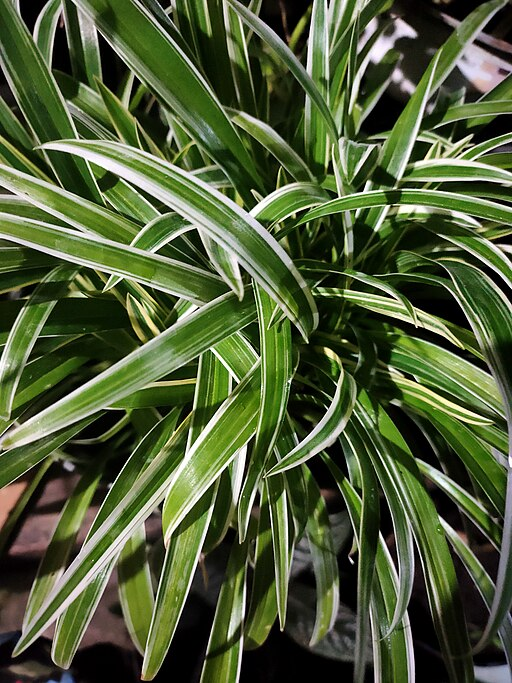
\includegraphics[width=\textwidth]{1_artificial_background.jpg}
                    \caption{\centering(\cite{1_artificial_background:2021})}
                \end{subfigure} &
                \begin{subfigure}{0.40\textwidth}
                    \centering
                    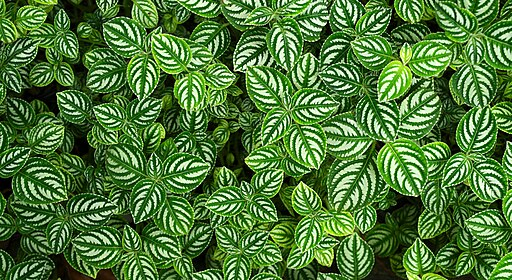
\includegraphics[width=\textwidth]{2_artificial_background.jpg}
                    \caption{\centering (\cite{2_artificial_background:2019})}
                \end{subfigure} &
                \begin{subfigure}{0.25\textwidth}
                    \centering
                    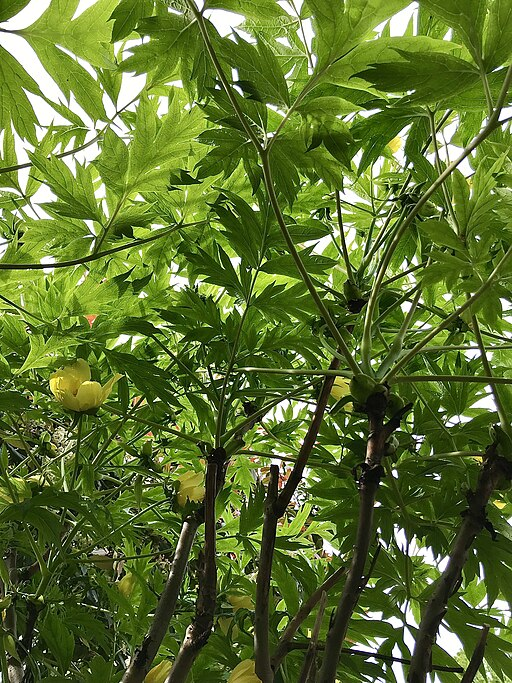
\includegraphics[width=\textwidth]{3_artificial_background.jpg}
                    \caption{\centering (\cite{3_artificial_background:2022})}
                \end{subfigure} \\
            \end{tabular}
            \begin{tabular}{ccc}
                \begin{subfigure}{0.30\textwidth}
                    \centering
                    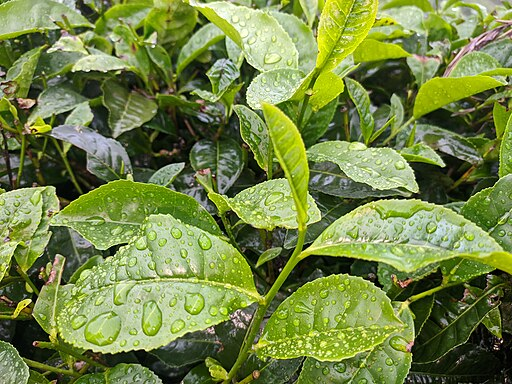
\includegraphics[width=\textwidth]{4_artificial_background.jpg}
                    \caption{\centering (\cite{4_artificial_background:2023})}
                \end{subfigure} &
                \begin{subfigure}{0.30\textwidth}
                    \centering
                    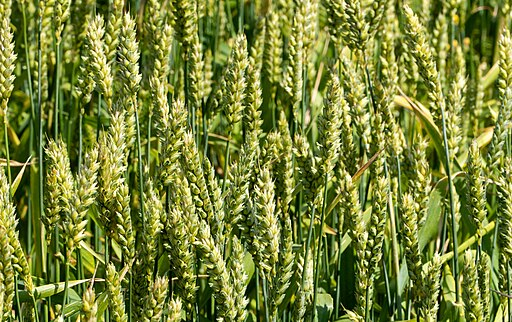
\includegraphics[width=\textwidth]{5_artificial_background.jpg}
                    \caption{\centering (\cite{5_artificial_background:2022})}
                \end{subfigure} &
                \begin{subfigure}{0.30\textwidth}
                    \centering
                    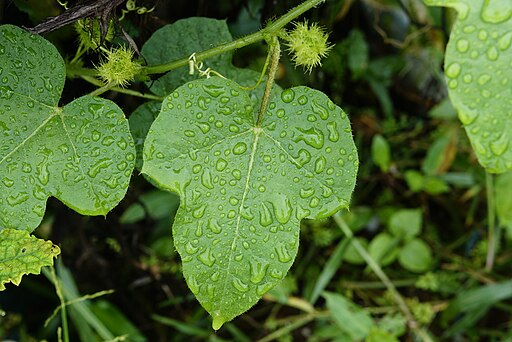
\includegraphics[width=\textwidth]{6_artificial_background.jpg}
                    \caption{\centering (\cite{6_artificial_background:2017})}
                \end{subfigure} \\
            \end{tabular}
            \begin{tabular}{ccc}
                \begin{subfigure}{0.30\textwidth}
                    \centering
                    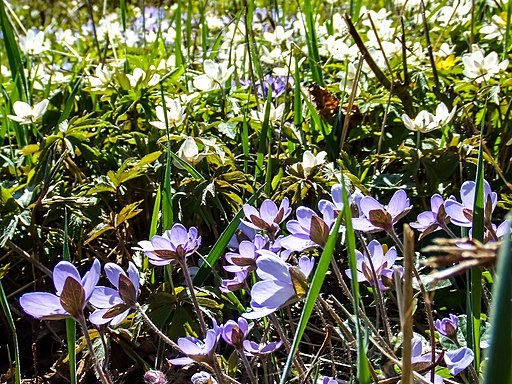
\includegraphics[width=\textwidth]{7_artificial_background.jpg}
                    \caption{\centering (\cite{7_artificial_background:2019})}
                \end{subfigure} &
                \begin{subfigure}{0.30\textwidth}
                    \centering
                    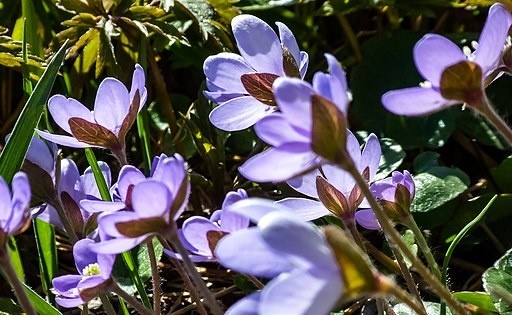
\includegraphics[width=\textwidth]{8_artificial_background.jpg}
                    \caption{\centering (\cite{8_artificial_background:2009})}
                \end{subfigure} &
                \begin{subfigure}{0.30\textwidth}
                    \centering
                    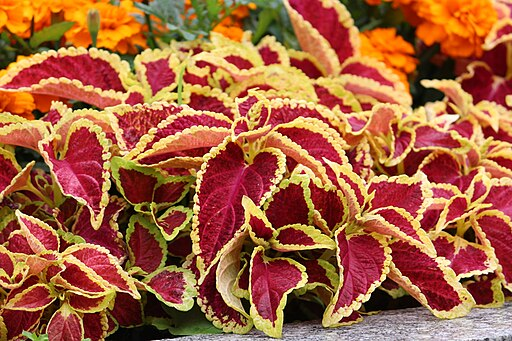
\includegraphics[width=\textwidth]{9_artificial_background.jpg}
                    \caption{\centering (\cite{9_artificial_background:2016})}
                \end{subfigure} \\
            \end{tabular}
            \begin{tabular}{c}
                \begin{subfigure}{0.30\textwidth}
                    \centering
                    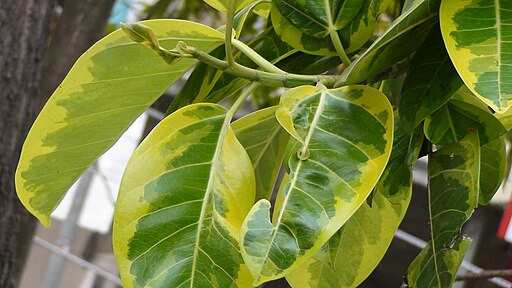
\includegraphics[width=\textwidth]{10_artificial_background.jpg}
                    \caption{\centering (\cite{10_artificial_background:2009})}
                \end{subfigure} \\
            \end{tabular}
            \caption{\centering Artificial background images used to augment the dataset}
            \label{fig:artificial-backgrounds}
        \end{figure}

        The initial dataset used for training a CNN model contained three subsets: color, segmented and artificial background. Because of computing resources constrains, the number of images per class in each subset of the initial dataset was limited to 400 images. \autoref{fig:dataset-image-examples} shows examples of images from each of the three subsets of the initial dataset.

        \begin{figure}[h]
            \centering
            \begin{tabular}{ccc}
                \begin{subfigure}[t]{0.30\textwidth}
                    \centering
                    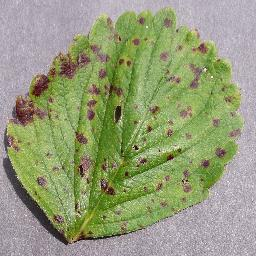
\includegraphics[width=\textwidth]{color_strawberry_leaf_scorch.JPG}
                    \caption{\centering Color subset}
                \end{subfigure} &
                \begin{subfigure}[t]{0.30\textwidth}
                    \centering
                    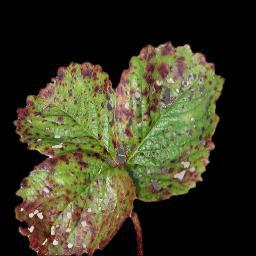
\includegraphics[width=\textwidth]{segmented_strawberry_leaf_scorch.jpg}
                    \caption{\centering Segmented subset}
                \end{subfigure} &
                \begin{subfigure}[t]{0.30\textwidth}
                    \centering
                    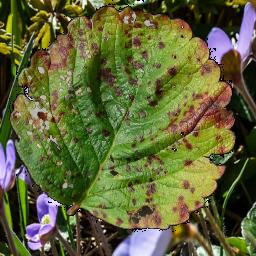
\includegraphics[width=\textwidth]{artificial_strawberry_leaf_scorch.jpg}
                    \caption{\centering Artificial background subset}
                \end{subfigure} \\
            \end{tabular}
            \caption{\centering Examples of images from color, segmented, and artificial background subsets}
            \label{fig:dataset-image-examples}
        \end{figure}

        \autoref{tab:dataset-overview} gives an overview of the initial dataset that was used to train and validate the CNN model. Each of the three subsets contains 14,731 images. In total, the whole initial dataset contains 44,193 images. Not limiting the size of the original dataset without the gray-scale subset, the dataset would contain almost 200,000 images.

        \begin{table}[h]
            \centering
            \begin{tabular}{@{}l|l|l|l|l|l@{}}
                \hline
                \multirow{2}{*}{Plant species} & \multirow{2}{*}{Plant disease} & \multicolumn{3}{c|}{Number of images} & \multirow{2}{*}{Total} \\ \cline{3-5}
                &  & Color & Segmented & Artificial &  \\ \hline
                \multirow{4}{*}{Apple} & Scab & 400 & 400 & 400 & 1,200 \\ \cline{2-6}
                & Black rot & 400 & 400 & 400 & 1,200 \\ \cline{2-6}
                & Cedar apple rust & 275 & 275 & 275 & 825 \\ \cline{2-6}
                & Healthy & 400 & 400 & 400 & 1,200 \\ \hline
                Blueberry & Healthy & 400 & 400 & 400 & 1,200 \\ \hline
                \multirow{2}{*}{Cherry} & Powdery mildew & 400 & 400 & 400 & 1,200 \\ \cline{2-6}
                & Healthy & 400 & 400 & 400 & 1,200 \\ \hline
                \multirow{4}{*}{Corn} & Cercospora leaf spot and Gray leaf spot & 400 & 400 & 400 & 1,200 \\ \cline{2-6}
                & Common rust & 400 & 400 & 400 & 1,200 \\ \cline{2-6}
                & Northern leaf blight & 400 & 400 & 400 & 1,200 \\ \cline{2-6}
                & Healthy & 400 & 400 & 400 & 1,200 \\ \hline
                \multirow{4}{*}{Grape} & Black rot & 400 & 400 & 400 & 1,200 \\ \cline{2-6}
                & Esca (Black measles) & 400 & 400 & 400 & 1,200 \\ \cline{2-6}
                & Leaf blight (Isariopsis leaf spot) & 400 & 400 & 400 & 1,200 \\ \cline{2-6}
                & Healthy & 400 & 400 & 400 & 1,200 \\ \hline
                Orange & Haunglongbing (Citrus greening) & 400 & 400 & 400 & 1,200 \\ \hline
                \multirow{2}{*}{Peach} & Bacterial spot & 400 & 400 & 400 & 1,200 \\ \cline{2-6}
                & Healthy & 360 & 360 & 360 & 1,080 \\ \hline
                \multirow{2}{*}{Pepper} & Bacterial spot & 400 & 400 & 400 & 1,200 \\ \cline{2-6}
                & Healthy & 400 & 400 & 400 & 1,200 \\ \hline
                \multirow{3}{*}{Potato} & Early blight & 400 & 400 & 400 & 1,200 \\ \cline{2-6}
                & Late blight & 400 & 400 & 400 & 1,200 \\ \cline{2-6}
                & Healthy & 152 & 152 & 152 & 456 \\ \hline
                Raspberry & Healthy & 371 & 371 & 371 & 1,113 \\ \hline
                Soybean & Healthy & 400 & 400 & 400 & 1,200 \\ \hline
                Squash & Powdery mildew & 400 & 400 & 400 & 1,200 \\ \hline
                \multirow{2}{*}{Strawberry} & Leaf scorch & 400 & 400 & 400 & 1,200 \\ \cline{2-6}
                & Healthy & 400 & 400 & 400 & 1,200 \\ \hline
                \multirow{9}{*}{Tomato} & Bacterial spot & 400 & 400 & 400 & 1,200 \\ \cline{2-6}
                & Early blight & 400 & 400 & 400 & 1,200 \\ \cline{2-6}
                & Late blight & 400 & 400 & 400 & 1,200 \\ \cline{2-6}
                & Leaf mold & 400 & 400 & 400 & 1,200 \\ \cline{2-6}
                & Septoria leaf spot & 400 & 400 & 400 & 1,200 \\ \cline{2-6}
                & Spider mite and Two-spotted spider mite & 400 & 400 & 400 & 1,200 \\ \cline{2-6}
                & Target spot & 400 & 400 & 400 & 1,200 \\ \cline{2-6}
                & Tomato yellow leaf curl virus & 373 & 373 & 373 & 1,200 \\ \cline{2-6}
                & Healthy & 400 & 400 & 400 & 1,200 \\ \hline
                Total &  & 14,731 & 14,731 & 14,731 & 44,193 \\ \hline
            \end{tabular}
            \caption{\centering Overveiw of the initial dataset}
            \label{tab:dataset-overview}
        \end{table}

        The images in the original dataset had the size of $256 \times 256$ pixels. Prior to the training process, the images of the initial dataset were divided into the train, test and validation datasets. To divide the initial dataset, the hold-out method was used. From the initial dataset, 80\% of the images were used in the training process. The train subset contained 35,349 images. The remaining 20\% of the images were used to validate the CNN model. The validation subset contained 8,844 images. Out of the images used for the training process, 80\% of the images were used for the actual training of the CNN and the rest of the images was used as test dataset. This test dataset was used to evaluate model's performance after each epoch. Furthermore, the images were resized to the input size of the CNN model trained. The input size of the CNN model trained was $224 \times 224$ pixels. To introduce more variability during the training process, the subset used for training of the CNN model was augmented using four different augmentation operations. These operation were: random horizontal and/or vertical flip, random rotation, random contrast incase or decrease, and random brightness increase or decrease. \autoref{fig:augmentation-pipeline} shows an image of a healthy Pepper leaf with artificial background and its different versions after applying the augmentation pipeline.

        \begin{figure}[h]
            \centering
            \begin{tabular}{ccc}
                \begin{subfigure}{0.30\textwidth}
                    \centering
                    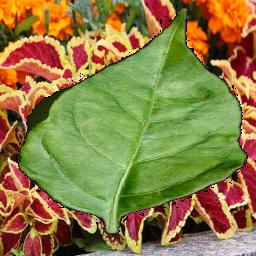
\includegraphics[width=\textwidth]{original_image.jpg}
                    \caption{\centering Original image}
                \end{subfigure} &
                \begin{subfigure}{0.30\textwidth}
                    \centering
                    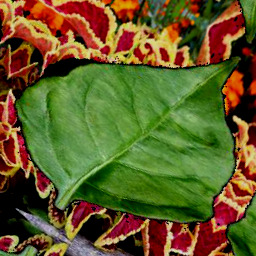
\includegraphics[width=\textwidth]{1_pipeline.png}
                    \caption{\centering Augmented image}
                \end{subfigure} &
                \begin{subfigure}{0.30\textwidth}
                    \centering
                    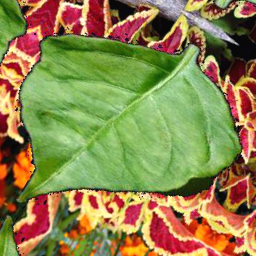
\includegraphics[width=\textwidth]{2_pipeline.png}
                    \caption{\centering Augmented image}
                \end{subfigure} \\
            \end{tabular}
            \begin{tabular}{ccc}
                \begin{subfigure}{0.30\textwidth}
                    \centering
                    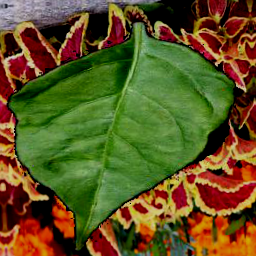
\includegraphics[width=\textwidth]{3_pipeline.png}
                    \caption{\centering Augmented image}
                \end{subfigure} &
                \begin{subfigure}{0.30\textwidth}
                    \centering
                    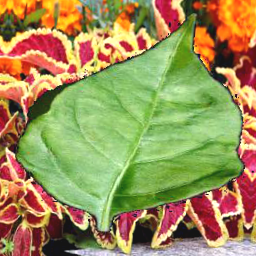
\includegraphics[width=\textwidth]{4_pipeline.png}
                    \caption{\centering Augmented image}
                \end{subfigure} &
                \begin{subfigure}{0.30\textwidth}
                    \centering
                    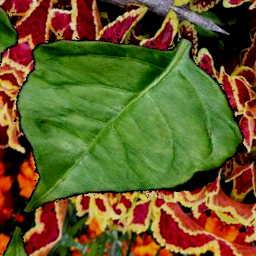
\includegraphics[width=\textwidth]{5_pipeline.png}
                    \caption{\centering Augmented image}
                \end{subfigure} \\
            \end{tabular}
            \caption{\centering Original image (Pepper healthy) and its different augmented versions}
            \label{fig:augmentation-pipeline}
        \end{figure}

        The various augmentation steps used in the dataset preprocessing introduce greater variability and complexity into the dataset used for the CNN model training and validation. However, the created dataset is significantly smaller than the dataset used by \textcite{Mohanty:2016}. Thus, it is very important to choose a CNN architecture that performs well enough when trained on the created dataset.

    \subsection{CNN Architecture} % EfficientB0 (from pretrained models in Keras)

    % A good rule of thumb is that the total number of training data points should be at least 2 to 3 times larger than the number of parameters in the neural network, although the precise number of data instances depends on the specific model at hand. In general, models with a larger number of parameters are said to have high capacity, and they require a larger amount of data in order to gain generalization power to unseen test data. The notion of overfitting is often understood in the trade-off between bias and variance in machine learning. (\cite{Aggarwal:2018})
                % when talking about the CNN model and the way to train it, I have to be talking about solver type, base learning rate, learning rate policy, Nesterov momentum, weight decay, gamma and batch size: \textcite{Mohanty:2016} \cite{Ferentinos:2018}
                % I can really test in on barbedo images even when training on plant village
                % \cite{Barbedo:2018:1}: parameters to train -> base learning rate, momentum, mini batch size, number of epochs,
        %\subsubsection{Model Architecture}
    \subsection{Training and Validation}
                % Instead, a widely adopted method known as n-fold cross-validation is used to exploit the labeled data both for model selection and for training. \cite{Mohri:2018} p 71
                % 4.3 Generalization Issues in Model Tuning and Evaluation (\cite{Aggarwal:2018}) -> Hold-Out vs. Cross-Validation
    \subsection{Web-based Application Design}
        \subsubsection{Frontend Design}
        \subsubsection{Backend Design}

\section{Development}
    \subsection{Dataset Preprocessing Pipeline}
    \subsection{CNN Model Training and Validation Package}
    % tensoflow and keras
    \subsection{Web-based Application Development}
        \subsubsection{Frontend Development}
        \subsubsection{Backend Development}

\section{Web-based Application Walkthrough}

\section{Discussion}
% Google Colab + Jupyter Notebook, training on my own computer then adding the plots

\section{Conclusion}

%----------------------------------------------------------------------------------------
% References
%----------------------------------------------------------------------------------------
\clearpage
\printbibliography

\end{document}
